%% 
%% Copyright 2019-2020 Elsevier Ltd
%% 
%% This file is part of the 'CAS Bundle'.
%% --------------------------------------
%% 
%% It may be distributed under the conditions of the LaTeX Project Public
%% License, either version 1.2 of this license or (at your option) any
%% later version.  The latest version of this license is in
%%    http://www.latex-project.org/lppl.txt
%% and version 1.2 or later is part of all distributions of LaTeX
%% version 1999/12/01 or later.
%% 
%% The list of all files belonging to the 'CAS Bundle' is
%% given in the file `manifest.txt'.
%% 
%% Template article for cas-dc documentclass for 
%% double column output.

%\documentclass[a4paper,fleqn,longmktitle]{cas-dc}
\documentclass[a4paper,fleqn]{cas-sc}

%\usepackage[numbers]{natbib}
%\usepackage[authoryear]{natbib}
\usepackage[authoryear,longnamesfirst]{natbib}
\usepackage{graphicx}
\usepackage{caption}
\usepackage{subcaption}
\usepackage{booktabs}
\usepackage{longtable}

%%%Author definitions
\def\tsc#1{\csdef{#1}{\textsc{\lowercase{#1}}\xspace}}
\tsc{WGM}
\tsc{QE}
\tsc{EP}
\tsc{PMS}
\tsc{BEC}
\tsc{DE}
%%%

% Uncomment and use as if needed
%\newtheorem{theorem}{Theorem}
%\newtheorem{lemma}[theorem]{Lemma}
%\newdefinition{rmk}{Remark}
%\newproof{pf}{Proof}
%\newproof{pot}{Proof of Theorem \ref{thm}}

\begin{document}
\let\WriteBookmarks\relax
\def\floatpagepagefraction{1}
\def\textpagefraction{.001}

% Short title
\shorttitle{Correspondence Analysis of Two-Mode Networks}

% Short author
%\shortauthors{O. Lizardo}

% Main title of the paper
\title [mode = title]{The Correspondence Analysis of Two-Mode Networks Revisited}                      
% Title footnote mark
% eg: \tnotemark[1]
%\tnotemark[1,2]

% Title footnote 1.
% eg: \tnotetext[1]{Title footnote text}
% \tnotetext[<tnote number>]{<tnote text>} 
%\tnotetext[1]{}

%\tnotetext[2]{.}


% First author
%
% Options: Use if required
% eg: \author[1,3]{Author Name}[type=editor,
%       style=chinese,
%       auid=000,
%       bioid=1,
%       prefix=Sir,
       %orcid=0000-0002-5405-3007,
%       facebook=<facebook id>,
%       twitter=<twitter id>,
%       linkedin=<linkedin id>,
%       gplus=<gplus id>]
%\author[1]{Omar Lizardo}[orcid=0000-0002-5405-3007]

% Corresponding author indication
%\cormark[1]

% Footnote of the first author
%\fnmark[1]

% Email id of the first author
%\ead{olizardo@soc.ucla.edu}

% URL of the first author
%\ead[url]{http://olizardo.bol.ucla.edu/}

%  Credit authorship
%\credit{Conceptualization of this study, Methodology, Software}

%Address/affiliation
%\affiliation[1]{organization={University of California, Los Angeles},
   % addressline={264 Haines Hall}, 
   % city={Los Angeles},
    %citysep={},  Uncomment if no comma needed between city and postcode
    % postcode={90095}, 
    % state={CA},
    % country={USA}}

 %Corresponding author text
%\cortext[cor1]{Corresponding author}
%\cortext[cor2]{Principal corresponding author}

%Footnote text
%\fntext[fn1]{This paper was written while the author was partially supported by National Science Foundation grant HNDS-R \#2214215.}
 % author as well.}
%\fntext[fn2]{Another author footnote, this is a very long footnote and
 % it should be a really long footnote. But this footnote is not yet
 % sufficiently long enough to make two lines of footnote text.}

% For a title note without a number/mark
%\nonumnote{This note has no numbers. In this work we demonstrate $a_b$
%  the formation Y\_1 of a new type of polariton on the interface
 % between a cuprous oxide slab and a polystyrene micro-sphere placed
 % on the slab.
 % }
% Here goes the abstract
\begin{abstract}
This paper reconsiders the use of Correspondence Analysis (CA) in analyzing two-mode network data, highlighting aspects that have not been previously emphasized and clarifying its linkages to two-mode centrality. I show that using CA to compute a dual score on both sets of nodes in a two-mode network is related to but not mathematically equivalent to the \citet{bonacich1991simultaneous} two-mode centrality. This ``reflective'' approach to computing dual scores connects the use of CA in two-mode network analysis to its use in other disciplines as a method of ordination. Additionally, I show that CA can extract latent positional information on people and groups, connecting it to recent work on extracting ``generalized relational similarities'' in two-mode networks. 
\end{abstract}

% Use if graphical abstract is present
% \begin{graphicalabstract}
% \includegraphics{figs/grabs.pdf}
% \end{graphicalabstract}

%Research highlights
\begin{highlights}
  \item This paper revisits the use of Correspondence Analysis (CA) in analyzing two-mode network data, highlighting its potential beyond data visualization.
  \item CA can compute a dual centrality score on both modes of a two-mode network, related to but not mathematically equivalent to the Bonacich (1991) two-mode centrality. 
  \item CA can extract latent positional information on people and groups, with similarities to recent work on generalized relational similarity" in two-mode networks. 
\end{highlights}

% Keywords
% Each keyword is separated by \sep
\begin{keywords}
Correspondence Analysis \sep Generalized Relational Similarity \sep Duality \sep Two-mode networks \sep Centrality 
\end{keywords}

\maketitle
\newpage
\section{Introduction} \label{sec:intro}
While not particularly common, using Correspondence Analysis---hereafter CA---in analyzing two-mode network data has had a somewhat rocky career in the social networks literature. Initially criticized by \citet{borgatti1997network} as a relatively limited and perhaps even inapplicable tool, CA has found various proponents who see it as an important component of the SNA arsenal for two-mode network data analysis, particularly regarding its ability to economically provide synoptic (e.g., ``joint'') graphical representations of structural connectivity patterns across the two-modes \citep{roberts2000correspondence, breiger2000tool, faust2005using}, with the primary aim being to use CA---or its variants like Multiple Correspondence Analysis (MCA)---to ``visually explore'' such networks \citep{desposito2014use}. 

 

\subsection{Organization of the Paper} \label{subsec:org}
The rest of the paper is organized as follows. In Section~\ref{sec:prevuses}, I review previous SNA work dealing with the uses of CA to analyze two-mode network data. Then, in Section~\ref{sec:ref2mode}, I consider a recent re-invention of CA (the economic complexity index) used to produce a type of Bonacich-style dual scoring via iterative scoring across the two modes of the affiliation matrix. This leads naturally to an abbreviated way of computing the same scores---CA and Bonacich---via spectral decomposition of the one-mode projection of the affiliation matrix for each set of nodes (degree-weighted in the case of CA and unweighted in the case of Bonacich). Section~\ref{sec:comparing} uses the classic Southern Women dataset to show the payoff of this approach, focusing on the distinct substantive insights extracted by CA and Bonacich scoring in a venerable dataset, showing that the CA-blocked affiliation matrix reveals a dual block partition between the two node sets (similar to that recovered by previous analyses of the same data using other methods), while the Bonacich-blocked affiliation recovers a core-periphery structure instead. In addition I show that considering higher dimensions of the Bonacich-style decomposition allows us to discover secondary core-periphery structures in the two-mode network, while also leading to a meaningful clustering of the nodes based on structural equivalence. Section~\ref{sec:cagensim} considers the hanging question of the exact substantive interpretation of the node clusters revealed by CA-style blocking, which are shown to be fairly close to those obtained by a computationally unrelated approach based on the idea of ``generalized relational similarity,'' suggesting that the CA blocks are distinct from those obtained following the logic of structural equivalence. Finally, Section~\ref{sec:disc} closes with a summary of key points in the argument and suggestions for future development of the linkages between CA and positional and centrality analysis in two-mode networks.  

\section{Previous uses of CA in Two-Mode Network Data Analysis} \label{sec:prevuses}

For reasons of space and relevance, my discussion of previous work is circumscribed in four ways, focusing on (1) pieces discussing primarily \textit{methodological} or interpretive aspects of CA, (2) regarding the analysis of \textit{two-mode network} data or affiliation networks,\footnote{There are, of course, various substantive applications of CA for the analysis of two-mode networks~\citep[e.g.,][]{breiger2000tool, faust2002scaling, schweizer1991power, serino2024mapping, ragozini2018analysis} as well as substantive and methodological applications of CA to the analysis of one-mode network data~\citep[e.g.,][]{noma1985scaling, kumbasar1994systematic, lizardo2020correspondence}; these will not be part of the discussion here.} (3) analyzing the usual \textit{binary} affiliation matrix measuring a single relation between persons and groups at one point in time, where links are observed only between persons and groups,\footnote{As such, recent work dealing with the application of CA or other factoring approaches to time-varying, multiplex, multilevel, or valued two-mode network data \citep{ragozini2014correspondence, ragozini2015multiple, zhu2016correspondence} will also be outside the scope of my discussion.} using with the \textit{simple CA} of the affiliation matrix.\footnote{There has been a spate of recent work focusing on the uses and advantages of using Multiple Correspondence Analysis or MCA---a variant of CA applied to a disjunctively-coded, doubly-centered version of the original affiliation matrix) to analyze and visualize two-mode networks \citep[e.g.,][]{dramalidis2016subset, desposito2014use, ragozini2014correspondence}. Because much of what I have to say deals with the uses and interpretation of the scores obtained from simple CA applied directly to the affiliation matrix (or its one-mode projections), my discussion will not be directly relevant to this line of work, except for a recent paper directly comparing the substantive interpretation of the $\chi^2$ distances in simple CA and MCA with regard to their substantive interpretation as indexes of structural similarity, which bears more directly to some of the subsequent discussion \citep{desposito2014comparison}.}

%With these restrictions in mind, the literature on CA, duality, and two-mode networks can be divided into two streams. The first contributions focus on the usefulness of CA as a tool for the visualization or ``joint display'' of the two sets of entities in an affiliation network. Secondly, some contributions focus on the similarities and differences between CA and factoring---those based on a spectral decomposition of a suitable matrix---techniques for assigning scores to the nodes of a two-mode network, where the scores exploit the duality between the two sets of entities and could be, under some circumstances, interpreted as ``centrality'' scores. 

\subsection{Previous Work on CA and Two-Mode Networks}
One of the earliest considerations of CA as a data-analytic tool for examining duality relations in two-mode networks was provided by \citet[163-165]{bonacich1991simultaneous} in his classic paper on dual centralities for affiliation networks. In that paper, \citet{bonacich1991simultaneous} noted that since the usual affiliation matrix is a ``cross-classification of people by the groups to which they belong,'' then it would seem that CA would be a relevant analytic technique. According to \citet{bonacich1991simultaneous}, the basic goal of correspondence analysis is to create a multidimensional space encoding geometric ``distances'' (scare quotes in the original) between row and column categories, with the distances capturing the best low-dimensional representation---in the least-squared error sense---of the similarities between row and column objects.  Bonacich's discussion of CA came after his influential introduction of the Eigenvector centrality approach for two-mode network analysis. Intriguingly, \citet[163]{bonacich1991simultaneous} noted that ``[a]lthough the goals of correspondence analysis and centrality analysis are different, their mathematics are similar,'' because both rely on a version of the spectral decomposition of the affiliation matrix---namely, the Singular Value Decomposition (SVD) to obtain scores for the row and column objects in the two-mode network. As we will see in section~\ref{subsec:refeigen}, CA and centrality analysis are mathematically linked in a second way not noted by Bonacich, as they are also based on the spectral decomposition of the dual one-mode \textit{projections} of the original rectangular affiliation matrix. In this particular respect, the mathematics connecting the Eigenvector approach to centrality analysis and CA are more similar than even Bonacich appreciated. 

For Bonacich, the main differences between CA and Eigenvector centrality analysis stemmed from ``the different ways in which the cross-classifications are treated before the SVD is applied.'' For Bonacich, the ``most powerful and useful dimensions'' of CA are designed to highlight and describe \textit{similarities} in row or column patterns of affiliation and membership, and therefore ``[b]efore the SVD is used, the cross-classification is modified so that these dimensions of similarity will be the most powerful.'' Nevertheless, Bonacich is not quite clear as to what this pre-modification amounts to, noting that given the fact that less ``powerful'' dimensions are usually discarded, it could be that among these ``there may be a dimension corresponding to centrality,'' but ``correspondence analysis is not designed to highlight this dimension.'' Interestingly, Bonacich went on to compute both the Eigenvector and CA scores for the canonical Southern Women data---which we will also do later in this paper---noting that ``[r]ather than centrality what\ldots[the CA scores] seem to capture is membership in the two cliques that attended different sets of events,'' with the magnitude of each woman and event score in the main dimension seeming to indicate the ``purity'' of their membership in each of the two cliques and for events; that is, the likelihood of being attended by their most representative members  \citep[164]{bonacich1991simultaneous}. 

In an influential paper on centrality in two-mode networks, \citet{faust1997centrality} returned to the issue of the connection between eigenvector centrality, CA, and dual relations between actors and events in two-mode networks. Faust noted that one thing both techniques had in common was that they both produced scores that truly exploited the duality of the two modes in the data. In the eigenvector case, this duality is strict, as the eigenvector centrality of a given person is the sum of the eigenvector scores of the event she attends; for events, their scores are given by the sum of the eigenvector centralities of its members. Importantly, \citet{faust1997centrality} noted that an exact parallel dual additive relationship was obtained between the CA scores corresponding to persons and groups. The CA score of a given person on a given dimension is the (weighted) sum of the scores in the same dimension of the events she attends. Similarly, for groups, the score on a given CA dimension is the (weighted) sum of the scores of the women who attend that event, a classic case of duality via mutual definition. %\citet{faust1997centrality} also specified the particular way that the affiliation matrix $\mathbf{A}$ had to be modified before applying the SVD (recall this is the step that creates the difference between CA and Eigenvector centrality), noting that each cell of the affiliation matrix is divided by the square root of the product of the number of events the row woman attends and the number of people attending the column event.

\citet{borgatti1997network} provided another early and influential in-depth consideration of CA in the context of two-mode network data analysis with an emphasis on the visualization aspect of actors and events in a single space. The discussion was placed in a section of the paper titled ``visual representations of 2-mode data,'' and naturally focused almost exclusively on the uses of CA as a visualization technique. According to \citet[246]{borgatti1997network}, CA ``can be seen as a method for representing points in a metric space such that distances between the points are meaningful.'' More specifically, \citet{borgatti1997network}, also using the Southern Women data as illustration,  claimed that in the CA map, points representing the women will appear closer if the women attend ``mostly the same events.'' Conversely, points representing the events will be placed near one another if the events were attended by ``mostly the same women,'' and that women and events would appear closer in the plot if ``those women attended those events.'' \citet[247-249]{borgatti1997network} then went on to focus on various limitations of CA as a visualization tool, noting that given the limiting range of dichotomous network data, two-dimensional representations ``will almost always be severely inaccurate or misleading.'' They also noted that since CA is a technique designed to deal with valued frequency data, its use with binary network data would lead to dimensional scores that would be either ``meaningless'' or ``difficult to interpret.'' Finally, they noted that since distances in the CA biplot are not Euclidean, they would mislead interpreters who would try to impose such a metric to make sense of them. 

In a paper published shortly thereafter, \citet{roberts2000correspondence} responded to some of the criticisms \citet{borgatti1997network} levied at the use of CA for analyzing two-mode networks. First, \citet{roberts2000correspondence} noted that there were many examples in the standing of using CA to analyze binary non-frequency data and that, therefore, the uses of CA are not constrained by the nature or provenance of the numerical quantities recorded in each cell of a two-mode network affiliation matrix. \citet{roberts2000correspondence} also challenged the contention that the two-dimensional representation of the data was unduly limiting in its capacity to produce a faithful representation of the original data, noting a high correlation between the distances between the women and the event points in the two-dimensional representation and one that used all thirteen dimensions.\footnote{In CA, the maximum number of dimensions is one minus the rank of the affiliation matrix, which in this case is fourteen, corresponding to the number of events.} Finally, \citet{roberts2000correspondence} also noted that the Euclidean distance interpretation of the separation of women and events points in the joint display is partially appropriate, as this Euclidean distances as actually low-dimensional approximations (to a high degree of accuracy in the first few dimensions) to the $\mathcal{X}^2$ distances between row profiles (for the women) and column profiles (for events) where the row profiles for a given woman is equal to the entry in the original affiliation matrix divided by the square root of the product of the number of events attended by that woman and the number of women who attended that event (and similarly for column profiles corresponding to events). Thus, the point distances are indeed interpretable as a kind of \textit{degree-weighted similarity} between objects in each mode. This is a point that we will return to later.   

Perhaps the most thorough discussion of the uses of CA as a tool for the dual ``joint display'' of affiliation networks is that provided by \citet{faust2005using}. According to \citet[118]{faust2005using}, previous debates regarding the usefulness---or lack thereof---of CA as a visualization tool were marred by imprecision and lack of ``formal specification'' regarding the exact substantive meaning of the scores obtained via the procedure and a related lack of sustained discussion as to the exact ``relationship between the model and the input data.'' Faust's basic point is that CA provides a way to both place actors and events in an affiliation network in a joint space such that the inter-point distances are interpretable and such that the link to the original data (e.g., the affiliation network matrix) is transparent. Along the way, \citet{faust2005using} established several important points. First, Faust specifies the exact matrix that is subject to the singular value decomposition when CA is applied directly to the affiliation matrix of a two-mode network $\mathbf{A}$; namely, a scaled version where $\mathbf{A}$ is pre-multiplied by a diagonal matrix containing the square root of its row sums and post-multiplied by a diagonal matrix containing the square root of its column sums. This is equivalent, as both \citet{faust1997centrality} and \citet{roberts2000correspondence} had noted before, to dividing every non-zero entry of $a_{pg}$ by the square root of the product of the number of memberships of person $p$ and the number of members of group $g$ before applying the SVD. Second, Faust specifies the exact relationship linking the resulting row and column CA scores and the original affiliation matrix input, providing the ``reconstruction equation'' that takes us from the left and right singular vectors and eigenvalues to the former. Thirdly, as she did in the 1997 two-mode centrality paper, Faust clarifies the duality linking the row and column scores, noting that the scores for the people are (activity) weighted sums of the scores that the groups they join, and the scores for the groups are (group size) weighted sums of the scores of their members. Finally, \citet[128ff]{faust2005using} clarifies the link between the CA scores---and different normalizations thereof---assigned to persons and events in an affiliation network on each dimension and (same node-set) inter-point distance in a joint space. Like \citet{roberts2000correspondence} before her, Faust specifies that in the low (usually two) dimensional representation, inter-point distances are best (least squares) approximations of the chi-square distance between the membership profiles of pairs of people (or groups), where the profile of a given person-row or group-column is equal to the non-zero entries of the affiliation matrix divided by the corresponding row or column sum (people's activities and group sizes).\footnote{Note that because the chi-square distances are defined on these degree-weighted entries, they define a kind of \textit{degree-weighted similarity} between pairs of people and pairs of groups, but not an exact similarity score as would be obtained, for instance, by using a criterion such as the proportion of matches in the affiliation matrix \citep[208]{everett2013dual}.}

In a recent paper, \citet{desposito2014comparison} compare CA and MCA as tools for representing the structural similarity between nodes in a two-mode network (actors in their case). Specifically, they analyze the significance of the typical $\chi^2$ distances defined from the scores obtained from the simple CA of the affiliation matrix as compared to the MCA of the indicator matrix of persons by groups with events treated as disjunctively coded binary variables measured over the actors (as just described). The focus of the analysis is the extent to which the $\chi^2$ distance of actor profiles obtained from the affiliation matrix $\mathbf{A}$ or the disjunctively coded indicator matrix $\mathbf{Z}$ best approaches a criterion for computing approximate structural equivalence between nodes (such as the Euclidean distance computed from the binary entries in the affiliation matrix).\footnote{In the case of MCA applied to the binary affiliation matrix, the latter is transformed into a new matrix $\mathbf{Z}$ with the same number of rows (persons) as the original and with twice the number of columns representing either membership ($z_{pg+} = 1$) or non-membership ($z_{pg-} = 1$) in that a group (disjunctive coding). The MCA scores are obtained via SVD of a centered and doubly normalized---with respect to person activity and group sizes---version of $\mathbf{Z}$ \citep{desposito2014use}.}  That is, \citet{desposito2014comparison} seek to ascertain whether CA or MCA is the best analytic tool to identify sets of \textit{structurally equivalent} actors in a two-mode network. 

Interestingly, \citet[115]{desposito2014comparison} note that just by examining the respective formulas defining the profile distances in CA versus MCA, we can verify that CA is \textit{not} a good tool for revealing clusters of structurally equivalent actors. As \citet{desposito2014comparison} put it, the reason is that the CA profile distance ``adopts a peculiar and more complex weighting system that could lead to a distorted representation of the actual relational patterns'' because the CA ``distance between actors (events) depends, not only on the pattern of participation (attendance)'' but also on the actor's \textit{degree} and the event \textit{sizes}. In addition, they note that because of this weighting scheme, in CA, ``small size events...are associated to larger weights...[and therefore] differences...related to such small size events have [a] stronger impact on the overall...distance than differences related to larger size events.'' \citet{desposito2014comparison} also point out that, in contrast, the MCA definition of inter-profile distance between actors based on $\mathbf{Z}$ is not affected by the degree-weighting aspect, and that in this respect, ``[I]t turns out that MCA [distances] closely resembles the Euclidean distance,'' which is a straightforward criterion for structural equivalence. This is a conclusion that is supported by computational experiments conducted later in the paper, and which leads \citet{desposito2014comparison} to conclude that the MCA defined  $\chi^2$ distances ``better reproduces the \textit{actual} relational pattern embedded in affiliation networks'' (122, italics added).

\subsection{Summary and Open Questions}
As we can see from this brief and necessarily selective review, considerations of CA for two-mode network analysis have generally intertwined two basic themes. One beginning with \citet{bonacich1991simultaneous} and continuing through \citet{faust1997centrality, faust2005using} have commented on the formal commonalities and contrasts between ``centrality analysis'' and ``correspondence analysis,'' noticing striking similarities in the mathematical formulations of the traditional dual (eigenvector) score and the scores obtained from CA, as both come from the eigendecomposition of the affiliation matrix, resulting in scores that meet the strict criterion for duality, as the scores of nodes in one mode are usually additive functions of the scores of nodes in the other mode. The other stream, which began with characterizations of CA as a visualization tool, focuses on the substantive meaning of the (low-dimensional representations of) the distances defined over the multidimensional space returned by the CA procedure. Here, multiple interpretations have been offered, from the idea that CA returns clique-like structures \citep{bonacich1991simultaneous}, to intimations that the closeness in the CA dimensions implies a more structured similarity closer to the idea of structural equivalence (e.g., such that actors that attend the same events and events that the same actors attend will be closer in the space). This approach sanctions the idea that the main goal of CA is to provide a parsimonious representation of the original ``input data'' \citep{faust2005using}, where this is understood to mean the original affiliation matrix. Yet, more recently, this line of interpretation has been controverted by  \citep{desposito2014comparison} who have noticed that whatever the CA similarities are designed to do, they are a less-than-optimal representation of structural equivalence (and thus presumably the original input data), given the specific weighting by the degree of nodes in each mode that is built into their construction. 

In one of the earliest and most comprehensive efforts introducing CA for the analysis of the composition and structure of relational data, \citet[19-21]{wasserman1990correspondence} noted that the history of CA in the social and behavioral sciences was one of invention, collective forgetting, and subsequent re-invention and independent rediscoveries, happening both within disciplines over time and across various fields of scholarly investigation at roughly contemporaneous intervals throughout the twentieth century.\footnote{As we will see in the next section, the pattern of CA reinvention and independent rediscovery continues into the twenty-first century, now involving disciplines outside the social and behavioral sciences narrowly conceived, including computer science, information science, and network science.} In the rest of the paper and starting in the next section, I show how a recent re-invention of CA for the analysis of ``economic complexity''---two-mode networks of countries/regions by the products they are most adept at producing---in the now well-established field of ``Network Science'' in the twenty-first century, allows us to revisit controversies and open questions as to the meaning of CA scores in two-mode network data, and the relationship between correspondence analysis, centrality analysis, and positional analysis (e.g., the discovery of structurally similar clusters of actors in two-mode networks). Along the way, we will be able to shed light on the link between CA scores and traditional eigenvector centrality scores for two-mode networks, as well as ascertain the exact kind of similarity that is learned by estimating CA (and traditional eigenvector centrality) scores for nodes in two-mode networks along multiple dimensions. 

\section{Reflective Node Scores in Two-Mode Networks} \label{sec:ref2mode}
In a highly cited piece, \citet{hidalgo2009building} motivated what they saw at the time as a novel way of assigning meaningful scores to nodes in a two-mode network using what they called at the time a ``reflective'' approach. Hidalgo and Hausmann's original empirical application was to the two-mode country-by-product networks. Hence, the original baptizing of their approach as one geared to extracting the ``economic complexity'' of countries in the world system (and dually the complexity of given products).\footnote{For a state-of-the-art review of the various substantive applications of the economic complexity approach see \citet{hidalgo2021economic}.} Subsequent work shows that there is no logical connection between the formal method and this particular application since the approach proposed can be used to analyze any two-mode data matrix. As such, I introduce it here using the more intuitive---and classical from a social network analysis perspective---case of the duality of persons and groups \citep{breiger1974duality}. This is consistent with the spirit of the original approach, recently described by \citet[92]{hidalgo2021economic} as centered on the ``\textit{duality} between economic inputs and outputs'' (italics mine).

If we are going to assign substantively meaningful scores to nodes in a two-mode network, the most natural place to start is with the good old \textit{degree centrality} \citep{faust1997centrality}. A two-mode network composed of a set of people $P$ and their affiliation relations to a set of groups $G$ can be represented by an affiliation matrix $\mathbf{A}$ of dimensions $|P| \times |G|$ with people along the rows and groups across the columns, where $|P|$ is the cardinality of the people set and $|G|$ is the cardinality of the group set, with cell entries $a_{pg}= 1$ if person \textit{p} is affiliated with group \textit{g} and $a_{pg}= 0$ otherwise. 

Given this, the degree-centrality of people is given by:

\begin{equation}
    C^R_p(1) = \sum_g a_{pg}
    \label{eq:R1_p}
\end{equation}

And for groups:

\begin{equation}
   C^R_g(1) = \sum_p a_{pg}
  \label{eq:R1_g}
\end{equation}

That is, the first-order centrality of people is the row sum of the entries in the affiliation matrix $\mathbf{A}$, and the column sums of the same matrix give the first-order centrality of groups. 

As noted by \citet{hidalgo2009building}, the key to the reflective approach to computing the ``complexity'' of countries and products is the observation that, once we have these first-order quantities, it is possible to compute ``second-order'' quantities $C^R(2)$ for both people and groups using the \textit{averaged} first-order centralities of the entities in the other mode they are connected to. 

For people, these are given by:

\begin{equation}
    C^R_p(2) = \frac{1}{C^R_p(1)}\sum_g a_{pg}C^R_g(1)
    \label{eq:R2_p}
\end{equation}

And for groups:

\begin{equation}
   C^R_g(2) = \frac{1}{C^R_g(1)}\sum_p a_{pg}C^R_p(1)
    \label{eq:R2_g}
\end{equation}

While Equation~\ref{eq:R1_p} assigns a high value to people who belong to a lot of groups, Equation~\ref{eq:R2_p} assigns a high value to people who, on average, belong to large groups (e.g., whenever $a_{pg} = 1$ and $C^R_g(1)$ is a big number). In the same way, while Equation~\ref{eq:R1_g} assigns a high value to groups that have lots of members, Equation~\ref{eq:R1_g} assigns a high value to groups that, on average, have members who themselves have lots of memberships (e.g., whenever $a_{pg} = 1$ and $C^R_p(1)$ is a big number). 

Of course, we can keep on going and define ``third-order'' reflections; for the people, these are given by:

\begin{equation}
   C^R_p(3) = \frac{1}{C^R_p(1)}\sum_g a_{pg}C^R_g(2)
   \label{eq:R3_p}
\end{equation}

And for groups:

\begin{equation}
   C^R_g(3) = \frac{1}{C^R_g(1)}\sum_p a_{pg}C^R_p(2)
   \label{eq:R3_g}
\end{equation}

As we saw, while for people, Equation~\ref{eq:R2_p} measured the average size of the groups they join, Equation~\ref{eq:R3_p} assigns a high value to people who, on average, belong to groups who are themselves attended by highly active members (e.g., whenever $a_{pg} = 1$ and $C^R_g(2)$ is a big number). In the same way, while Equation~\ref{eq:R2_g} assigns a high value to groups whose members have lots of memberships, Equation~\ref{eq:R3_g} assigns a high value to groups that, on average, have members who themselves (also on average) belong to large groups (e.g., $a_{pg} = 1$ and $C^R_p(2)$ is a big number).

Note that for the people, the even-numbered reflection $C^R_p(2)$ assigns centrality based on a formal feature of the \textit{groups} they belong to (in this case, the group sizes). On the other hand, the odd-numbered reflection $C^R_p(3)$ assigns centrality based on a formal feature of the \textit{members of the groups} they belong to (in this case, the average size of the groups they belong to). In the same way, for the groups, the even-numbered reflection $C^R_g(2)$ assigns centrality based on a formal feature of the \textit{people} who belong to them (in this case, their activity). On the other hand, the odd-numbered reflection $C^R_g(3)$ assigns centrality based on a formal feature of the \textit{other groups their members belong to} (in this case, their average group size). While these are distinct metrics, in practice, the ordering of the nodes in each mode ends up being identical across even and odd centralities after the ranks ``freeze'' past a given number of iterations (proportional to the network size). 

More generally, \citet{hidalgo2009building} show that we can define a series of reflective quantities for people and groups (whose verbal and substantive interpretation becomes more complex as the number of iterations increases). 

For people, these are given by:

\begin{equation}   
    C^R_p(q) = \frac{1}{C^R_p(1)}\sum_g a_{pg}C^R_g(q-1) 
   \label{eq:Rq_p}
\end{equation}

And for groups:

\begin{equation}
   C^R_g(q) = \frac{1}{C^R_g(1)}\sum_p a_{pg}C^R_p(q-1)
   \label{eq:Rq_g}
\end{equation}

Equation~\ref{eq:Rq_p} says that the reflective score of a person \textit{p} at iteration \textit{q} is the sum of the $q-1$ centralities of the groups they belong to ($C^R_g(q-1)$) divided by their number of memberships $C^{R}_p(1)$. Equation~\ref{eq:Rq_g} says that the $q^{th}$ group reflective score is the sum of $q-1$ centralities $C^R_p(q-1)$ of their members, divided by the number of group members $C^R_g(1)$.

\begin{figure}[ht!]
    \captionsetup[subfigure]{font=footnotesize,labelfont=footnotesize}
    \centering
    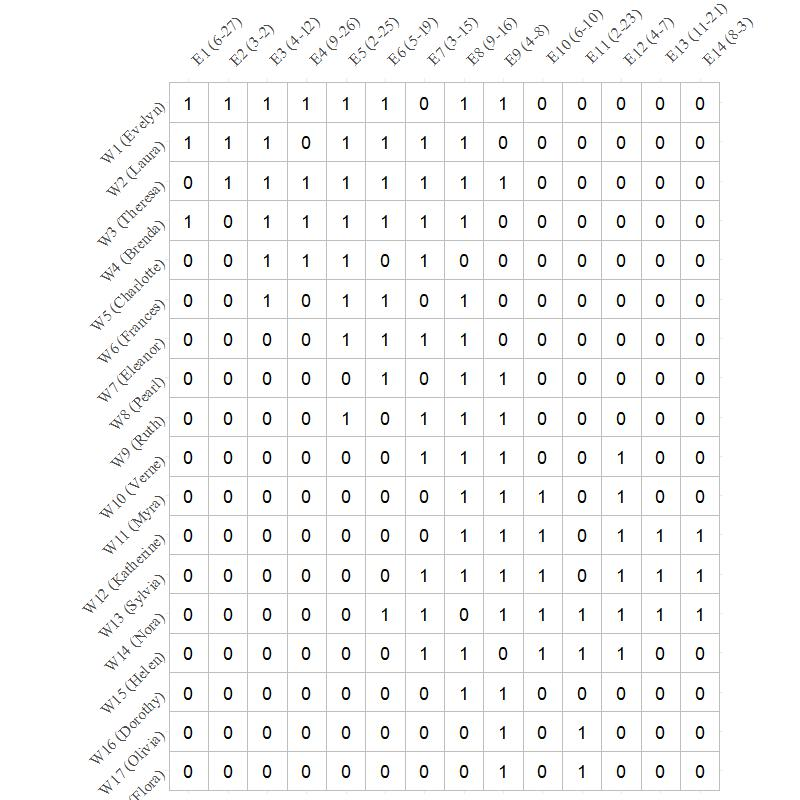
\includegraphics[width=0.65\textwidth]{Plots/southern-women.jpg}
    \caption{Southern Women data matrix with rows and columns ordered as in the original DGG table.}
    \label{fig:sw}
\end{figure}

\subsection{Empirical Example} \label{subsec:ex}
\subsubsection{Southern Women Data}
The following analyses use the classic ``Southern Women'' data \citep{davis1941} (DGG) as the running example. This data is doubly appropriate for showcasing the relevance of methods that exploit the duality between two sets of entities, as it was used in Breiger's \citeyearpar{breiger1974duality} classic paper. Moreover, Southern Women is a dataset that, according to \citet[p.]{freeman2003finding}, ``has become something of a touchstone for comparing analytic methods in social network analysis,'' having been analyzed ``again and again,'' and reappearing ``whenever any network analyst wants to explore the utility of some new tool for analyzing data.'' Freeman himself would go to review twenty-one such attempts. The list has only gotten much longer in the last two decades since Freeman's methodological ``meta-analysis'' \citep[e.g.,][among many others]{doreian2004generalized, field2006identifying, roffilli2006identifying, wang2009exponential, kovacs2010generalized, brusco2011analysis, borgatti2014analyzing, everett2013dual, lerner2022dynamic, batagelj2022analysis, lizardo2024two}. Despite this long list of studies of the Southern Women data, we will see that novel insights can still be garnered from this old data source.

Despite its undisputed pedigree as a methodological touchstone in studies of duality and dual constitution in two-mode networks, a key source of confusion in the mini-literature that exists around the Southern Women data concerns the order of presentation of the rows and columns. The reason for this is while the row mode (people) is ``nominal'' in both the scaling and the literal senses (being composed of women's names), the column mode (events) is more ambiguous. It \textit{could} be treated as nominal; however, the original DGG table includes event \textit{dates}, which means that it could also be treated as having a natural ordering, which could be reflected in the way we list the columns.  As \citet{freeman2003finding} notes, in the canonical original table included in \citet{davis1941}, both the row and column modes had been re-ordered in a presentation to reveal what DGG ascertained (using intuitive methods and in-depth knowledge of the case) was the group structure among the women; this means that the events were \textit{not} presented in chronological order from left to right across the columns. 

To add to the confusion, the original DGG table added arbitrary ordered numerical designators to both people and events, such that people came to refer to ``W1'' or ``W11'' and ``E1'' or ``E13'' based on the original DGG ordering, which may not have mattered for the women, but it mattered for the events because ``E14'' in the original DGG data is not the last chronological even among the fourteen columns. In fact, as shown in Figure~\ref{fig:sw}, it is the event that occurred on August 3rd, and three events occurred after that (E4, E8, and E13) in the DGG numbering.\footnote{Using the DGG labeling, the chronologically ordered set of events are \{E11, E5, E2, E7, E12, E9, E3, E6, E10, E1, E14 E8, E4, E13\} \citep[p. 68]{everett2018measuring}.} To further add to the confusion, some early analyses of the data, including Breiger's \citeyearpar{breiger1974duality} classic article and \citet{doreian1979evolution} used a \textit{different} ordering of the women---taken from \citet[83]{homans1950human}---from that of the original DGG table reproduced in \citet{freeman2003finding}, and ordered the events from left to right in the affiliation matrix \textit{chronologically}, which, as we have seen, also differs from the original DGG Table reproduced in \citet{freeman2003finding}. This means that the arbitrary ordinal labeling of the rows (e.g., ``W1,'' ``W2,'' ``W3,'' etc.) and the columns (e.g., ``E1,'' ``E2,'' ``E3,'' etc.) in these (and other) publications---see, e.g., \citep[table 1]{doreian1979evolution}---does not correspond to the DGG ordering reproduced in \citet{freeman2003finding} and more recent publications \citep[e.g.,][]{borgatti2014analyzing, batagelj2022analysis}; in all, different versions of the dataset reproduce different versions of the labeling. 

Of course, the specific labeling of the nodes does not really matter since we are usually interested in the structural properties of the rows and columns. Event ordering, however, matters for analyses that try to exploit the temporal properties of the data \citep[e.g.,][]{everett2018measuring, lerner2022dynamic}. Less substantively, but still importantly, the labeling of both the rows and columns does matter when trying to reconcile claims across publications from the narrative included in various papers, since ``W1'' or ``E8'' in one publication \citep[e.g.,][]{freeman2003finding} may not correspond to ``W1'' or ``E8'' in the other \citep[e.g.,][]{doreian1979evolution}. To forestall confusion, in what follows, I use the numeric labeling corresponding to the original DGG data table as reproduced in (among others) \citet[Figure 1]{freeman2003finding} and \citet[Figure 28.1]{borgatti2014analyzing}, and shown in Table~\ref{fig:sw}. My presentation includes both the arbitrarily ordered labels (e.g., ``W1'' or ``E1'') and both the woman's name and the event date in parentheses, with ``Myrna'' (W11) rebaptized to her given name of ``Myra'' to correspond to the original DGG table \citep{freeman2003finding, batagelj2022analysis}.

\subsubsection{Reflective Score Trajectory}
Figure~\ref{fig:p-refs} shows the trajectory of the HH reflective scores for persons, using a bump chart to plot the rank order trajectory of persons across reflections. The rank order of people and groups in the $q^{th}$ centrality is plotted on the y-axis, and the centrality iteration $q$ is plotted on the x-axis. As the figure shows, $NORA$, $FLORA$, $CHARLOTTE$, and $EVELYN$ are the top-ranked actors when it comes to $C^R_p(2)$:  The average number of members of the groups they belong to. However, their fates in this reflective metric diverge at higher reflections, with $NORA$ and $FLORA$ maintaining their top positions but $CHARLOTTE$ and $EVELYN$ tumbling down the ranks, suggesting that the members of the groups they belong to affiliate with smaller groups than the members of the groups $NORA$ and $FLORA$ belong to (and so on for higher reflections). 

In the exhaustive methodological meta-analysis mentioned earlier, \citet{freeman2003finding} noted that ``the consensus of the analytic procedures is to assign women 1 through 9 to one group and women 10 through 18 to the other.'' Notably, the reflective score rankings after freezing ($q \geq 18$) recover this same dominant partition reading from top to bottom. Figure~\ref{fig:g-refs} shows the corresponding bump chart for the events.  Clearly, $E14$ experiences the most dramatic improvement in status as we move to higher reflections. Relatively low ranked when it comes to the average number of memberships of its members, it increases in standing when considering (the average of) the average number of memberships of its members (and so forth). Notably, the equilibrium reflective scores recover and ordering of groups columns that re-appears across many articles that have analyzed these data with events 1-6 separated from events 10-15 by events 7-9 \citep[see e.g.,][]{doreian2004generalized, kovacs2010generalized, lizardo2024two, everett2013dual}.

\begin{figure}[ht!]
    \captionsetup[subfigure]{font=footnotesize,labelfont=footnotesize}
    \centering
     \begin{subfigure}[b]{0.45\textwidth}
        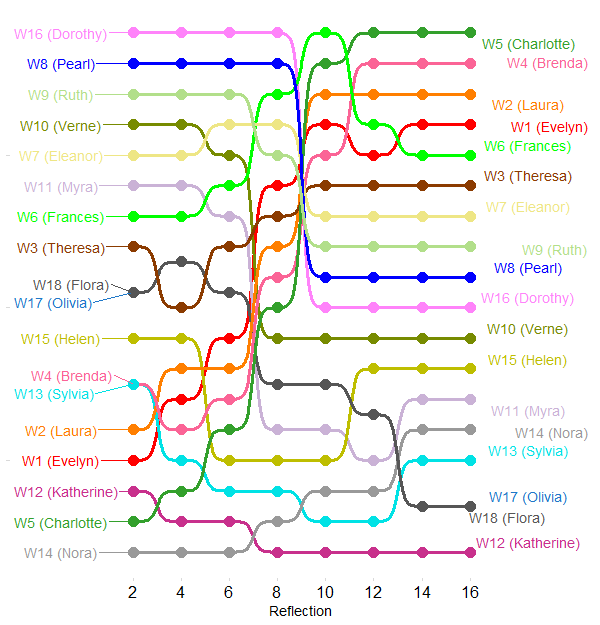
\includegraphics[width=1.0\textwidth]{Plots/p-reflections.png}
            \caption{Reflective score trajectories of persons.}
            \label{fig:p-refs}
    \end{subfigure}
     \begin{subfigure}[b]{0.45\textwidth}
        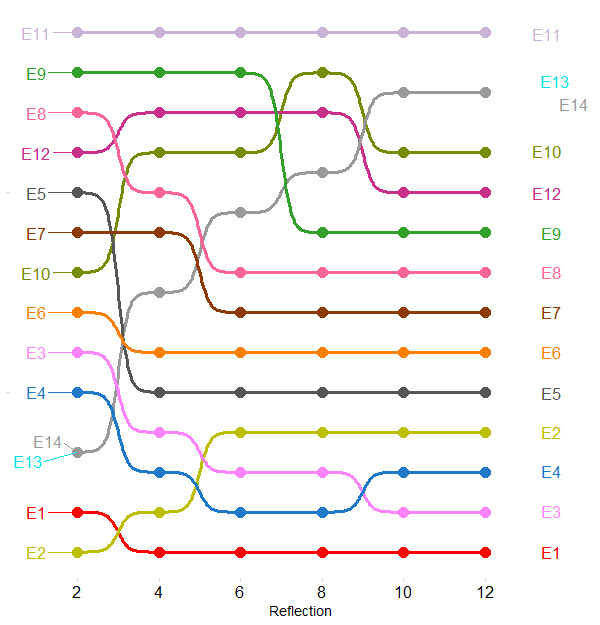
\includegraphics[width=1.0\textwidth]{Plots/g-reflections.png}
            \caption{Reflective score trajectories of groups.}
            \label{fig:g-refs}
    \end{subfigure}
    \caption{Reflective scores for persons and groups (even reflections)}
    \label{fig:refs}
\end{figure}

\subsection{CA and Dual Centrality Scoring in Two-Mode Networks} \label{sec:ca}
The reader may ask what the point of going through all this reflective scoring is since \citet{bonacich1991simultaneous} already developed a dual approach to scoring nodes in two-mode networks based on a very similar idea: Define the scores of entities in one mode based on the scores of entities in the other mode to which they are connected. As we have already noted, Bonacich also considered CA in passing as a possible technique to assign scores to nodes in a two-mode network but (perhaps rightly) dismissed it as producing scores that could be interpreted as a kind of ``centrality,'' noting that it was better at capturing the clique structure of women who attended different events \citeyearpar[164]{bonacich1991simultaneous}. 

While using CA to capture patterns of similarity in attendance between persons and groups makes sense (although, as we will see, the exact patterns of similarity captured by CA are not reducible to ``cliques'' as traditionally understood), CA can also be used to assign meaningful scores to nodes in a social network, which in some applications may even be interpreted as a type of centrality (or at least have a specifiable mathematical relation to scores that are usually unambiguously interpreted as centrality measures). In fact, as I will show in a bit, in the two-mode case, the first CA dimension captures the limit $(q \rightarrow \infty)$ of the reflective scores discussed in the previous section \citep{mealy2019interpreting}. This makes the connection between the Bonacich and the CA scoring approaches more intimate than Bonacich thought. 

To begin to see the linkages between CA and the Bonacich approach, recall that the solutions to the following system of linear equations give the Bonacich $(C^B)$ two-mode centralities:

\begin{equation}
    \mathbf{A}C^B_p = \lambda C^B_g 
    \label{eq:bon1}
\end{equation}

\begin{equation}
    \mathbf{A}^TC^B_g = \lambda C^B_p 
    \label{eq:bon2}
\end{equation}

Where $\mathbf{A}$ is the original affiliation matrix. Equations~\ref{eq:bon1} and~\ref{eq:bon2} have the typical form of a linear eigensystem, which means the unknown $C^B_g$ and $C^B_p$ scores can be obtained from the row and column eigenvectors corresponding to the largest eigenvalue $\lambda_1$, after performing a singular value decomposition (SVD) of the rectangular affiliation matrix $\mathbf{A}$. 

Importantly, as Faust \citeyearpar[170]{faust1997centrality} notes, it is possible to express Equations~\ref{eq:bon1} and~\ref{eq:bon2} in terms of person and group-specific scores; for people, these are given by: 

\begin{equation}
    C^B_p = \frac{1}{\lambda_1}\sum_{g}a_{pg}C^B_g
    \label{eq:faust1}
\end{equation}

And for groups:

\begin{equation}
    C^B_g = \frac{1}{\lambda_1}\sum_{p}a_{pg}C^B_p
    \label{eq:faust2}
\end{equation}

Where $\lambda_1$ is the largest (first) eigenvalue corresponding to the eigenvector containing the $C^B_p$ scores. These equations make clear that in the Bonacich dual-scoring approach, the scores assigned to people are equal to the sum of the scores of the groups they join, and the scores assigned to groups are equivalent to the sum of the scores simultaneously assigned to their members. This approach thus nicely captures the duality property since the scores of nodes in each mode are given by aggregating their connections to nodes in the other mode. 

Note, however, the formal similarity between equations~\ref{eq:faust1} and~\ref{eq:faust2} and equations~\ref{eq:Rq_p} and~\ref{eq:Rq_g}. The main difference is that in HH's reflective equations, a person's centrality is proportional to the \textit{group-degree-weighted} centralities of the groups they join, and a group's centrality is proportional to the \textit{person-degree-weighted} centrality of the people who are members. We will return to this crucial point later.

\subsection{Bonacich Reflections} \label{subsec:bonref}
We can motivate the Bonacich eigenvector-based approach using the same ``reflective'' exposition we used to introduce the HH reflective approach in Section~\ref{sec:ref2mode}. Admittedly, this is a somewhat unorthodox way of presenting the eigenvector centralities for two-mode networks; but it will help clarify the similarities and differences between the HH and the Bonacich approaches. 

Accordingly, starting with Equations~\ref{eq:R1_p} and~\ref{eq:R1_g}, we can define a second-order ``Bonacich-reflection'' on both the persons and groups using the formulas:

\begin{equation}
   C^B_p(2) = \sum_g a_{pg}C^R_g(1)
   \label{eq:BR2_p}
\end{equation} 

\begin{equation}
   C^B_g(2) = \sum_p a_{pg}C^R_p(1)
   \label{eq:BR2_g}
\end{equation}

Equation~\ref{eq:BR2_p} says that people are central when the sum of the number of members of the groups they belong to is large. Equation~\ref{eq:BR2_g} says groups are central when the sum of the number of memberships of the people who belong to them is large. 

As before, we can keep on going and define a third-order reflection using the formulas:

\begin{equation}
   C^B_p(3) = \sum_g a_{pg}C^R_g(2)
   \label{eq:BR3_p}
\end{equation} 

\begin{equation}
   C^B_g(3) = \sum_p a_{pg}C^R_p(2)
   \label{eq:BR3_g}
\end{equation}

Equation~\ref{eq:BR3_p} says that people are central when the sum of the sum of the number of memberships held by the people who belong to the groups they belong to is large. Equation~\ref{eq:BR3_g} says that groups are central when the sum of the sum of the number of members of the groups their members belong to is large. Once again, we can keep going and define fourth order, fifth order, and higher reflections $C^R_p(4), C^R_p(4) \ldots C^R_p(q)$, where the centralities of nodes in one mode are based on the sums, of the sums, of the sums, of the centralities of nodes in the other mode.

More generally, and in parallel with equations~\ref{eq:Rq_p} and~\ref{eq:Rq_g}, the reflective Bonacich centralities for persons and groups are given by:

\begin{equation}
   C^B_p(q) = \sum_g a_{pg}C^R_g(q-1)
   \label{eq:BRq_p}
\end{equation} 

\begin{equation}
   C^B_g(q) = \sum_p a_{pg}C^R_p(q-1)
   \label{eq:BRq_g}
\end{equation} 

This says that the Bonacich reflection at step $q$ is just the sum of the group centralities at step $q-1$ (for people) and the sum of the person centralities at step $q-1$ (for groups). Of course, these sums of sums would diverge to a larger and larger quantity at each step $q$. To prevent this and guarantee convergence, we can normalize the vector of reflective Bonacich centralities for persons and groups at each step $q > 1$ before calculating the subsequent sum at step $q+1$ as follows:

\begin{equation}
   C^B_p(q) = \frac{C^B_p(q)}{||C^B_p(q)||_2}
   \label{eq:BRq_pn}
\end{equation} 

\begin{equation}
   C^B_g(q) = \frac{C^B_g(q)}{||C^B_g(q)||_2}
   \label{eq:BRq_gn}
\end{equation} 

Where the denominator in~\ref{eq:BRq_pn} and~\ref{eq:BRq_gn} is the Euclidean vector norm.\footnote{For any vector $\mathbf{x}$ of length $n$, the $L_2$ norm is given by: $||\mathbf{x}||_2 = \sqrt{\sum_i^n x_i^2}$.} The normalization will prevent divergence of the sum of centralities for persons and groups, formalizing the weaker assumption of \textit{proportionality} between the centrality of each set of nodes and the sum of the centralities of the nodes in the other mode to which they are connected rather than the stronger assumption of strict equivalence \citep{bonacich_lloyd01}. Furthermore, the normalization guarantees convergence and the ``freezing'' of the sums of sums around steady values after a few iterations. These values will be equivalent (up to rounding error) to the (absolute value) of the dominant row and column eigenvectors of $\mathbf{A}$ as given in~\ref{eq:bon1} and~\ref{eq:bon2}.\footnote{Note that dividing by any vector norm---e.g., the $L_1$ or max norm---will prevent divergence and return scores perfectly correlated to the Bonacich eigenvector approach. Dividing by the $L_2$ norm returns scores that are \textit{exactly} the same, save for rounding error, as the absolute value of the dominant left and right eigenvectors of the affiliation matrix.} In fact, the iterative (normalized sum of sums) approach is one way of computing the leading eigenvectors of a rectangular matrix (e.g., the ``power method'' of \citet{mises1929praktische}). 

This exercise establishes that there is more than a superficial similarity between the HH ``reflective'' scores and the Bonacich two-mode eigenvector centralities. In fact, both can be seen as instantiating an underlying ``prismatic'' model---in the sense of \citet{podolny2001networks}---of how centrality is distributed in the two-mode network. The Bonacich approach, based on sums of sums, favors overall \textit{volume}---or two-mode ``total effects'' in the sense of \citet{friedkin1991theoretical}---thus, groups receive more centrality points from their more central members and fewer centrality points from their less central members. Likewise, people receive more centrality points from their more central memberships and fewer centrality points from their less central memberships, and so on through every iteration. The HH reflective approach (and CA by implication) favors \textit{averages} rather than volume; thus, a person with a few memberships can contribute as much centrality to the group they belong to as a person with many memberships if the person with fewer memberships belongs to (on average) more central groups and the person with more memberships belongs to (on average) less central ones. In the same way, a person can receive as much centrality from a small group they belong to compared to a large group, as long as the small group (on average) has more central members in it, and the large group (on average) has less central members.  

\subsection{HH Reflections as Correspondence Analysis} \label{subsec:refeigen}
Since iterating through normalized sums of sums is one way of obtaining the Bonacich two-mode centralities, it would be surprising if the equilibrium values of the HH reflective iterations were not themselves the solution to some eigenvalue decomposition problem. As has been noted recently by \citet{mealy2019interpreting} and \citet{van2021correspondence}, the Hidalgo and Hausmann's \citeyearpar{hidalgo2009building} reflective scores can indeed be obtained directly (without iterations) as the solution to an eigenvalue decomposition problem. 

To see this, recall that, as Bonacich \citeyearpar[157]{bonacich1991simultaneous} notes, we can solve for $C^B_g$ in~\ref{eq:bon2} and $C^B_p$ in~\ref{eq:bon1} and substitute the respective solutions into \ref{eq:bon1} and~\ref{eq:bon2}. Matrix-algebraic reduction of the resulting equations would show that the Bonacich dual centralities can also be obtained as solutions to the eigensystem:

\begin{equation}
    \left(\mathbf{AA}^T\right)C^B_p = \lambda C^B_p
    \label{eq:bon3}
\end{equation}

\begin{equation}
    \left(\mathbf{A}^T\mathbf{A}\right)C^B_g = \lambda C^B_g
    \label{eq:bon4}
\end{equation}

This shows that the dual centrality Bonacich scores for persons and groups are equivalent to the eigenvectors of the respective one-mode ``Breiger'' \citeyearpar{breiger1974duality} projection matrices corresponding to the first (largest) eigenvalue, which qualifies the Bonacich scores as a ``dual projection'' method for analyzing two-mode networks in the sense of \citet{everett2013dual}.

We can motivate CA using the same dual projection strategy. Typically, when CA is presented as the solution to an eigenvalue problem, this is done by showing how the relevant scores can be obtained via the singular value decomposition (SVD) of the rectangular affiliation matrix~\citep{borgatti1997network, bonacich1991simultaneous, faust1997centrality, faust2005using}. This gives the impression that CA is exclusively a ``direct'' rather than a dual projection method. Here, we will show that CA can also be motivated, and scores obtained via a similar ``dual'' projection approach just like the Bonacich eigenvector scores, except that these are scores associated with a \textit{degree-weighted} projection of the original affiliation matrix.

To see this, consider the $|P| \times |P|$ matrix $\mathbf{D}p$, containing the ``first order'' reflective scores of each person $C^R(1)_p$ (activity) along the diagonals and zeroes in every other cell. In the same way, consider the $|G| \times |G|$ matrix $\mathbf{D}g$, which contains the ``first order'' (degree) centralities of each group $C^R(1)_g$ (size) along the diagonals and zeroes in every other cell. Using these matrices, we can compute \textit{row stochastic} versions of the affiliation matrix and its transpose.\footnote{Recall that a matrix is row stochastic if its rows sum to one} For the people, we can do this by taking the original affiliation matrix and pre-multiplying it by $\mathbf{D}p^{-1}$ (which now contains the \textit{inverse} of the first-order centralities of each person $C^R_p(1)$ along the diagonals), yielding the row-stochastic matrix $\mathbf{P}_{pg}$ of dimensions $|P| \times |G|$:

\begin{equation}
    \mathbf{P}_{pg} = \mathbf{D}p^{-1}\mathbf{A}
    \label{eq:ca1}
\end{equation}

We can do the same with the groups, except that we pre-multiply the \textit{transpose} of the original affiliation matrix by $\mathbf{D}g^{-1}$ (which now contains the \textit{inverse} of the first-order centralities of each group $C^R_g(1)$ along the diagonals) yielding the row-stochastic matrix $\mathbf{P}_{gp}$ of dimensions $|G| \times |P|$:

\begin{equation}
    \mathbf{P}_{gp} = \mathbf{D}_G^{-1}\mathbf{A}^T
    \label{eq:ca2}
\end{equation}

Both $\mathbf{P}_{pg}$ and $\mathbf{P}_{gp}$ are just centrality-weighted versions of the original affiliation matrix and its transpose; accordingly, nothing is stopping us from proceeding with the usual next step---due to \citet{breiger1974duality}---of calculating the degree-weighted \textit{projections} for people and groups from these matrices. 

For the people, the degree-weighted projection is:

\begin{equation}
\mathbf{P}_{pp} = \mathbf{P}_{pg}\mathbf{P}_{gp}
    \label{eq:ca3}
\end{equation}

And for the groups:

\begin{equation}
    \mathbf{P}_{gg} = \mathbf{P}_{gp}\mathbf{P}_{pg}
    \label{eq:ca4}
\end{equation}

Both $\mathbf{P}_{pp}$ and $\mathbf{P}_{gg}$ are square ($|P| \times |P|$ and $|G| \times |G|$) respectively) degree-normalized projection matrices linking people and groups. Like their constituent matrices, both $\mathbf{P}_{pp}$ and $\mathbf{P}_{gg}$ are row-stochastic (rows constrained to sum to 1.0), positive definite, but not symmetric, as can be seen in Figure~\ref{fig:dwproj}. Interestingly, one way to interpret the entries in the degree-weighted projection matrices for people and groups is by giving the \textit{probabilities} that a random walker starting at the row person (group) and, following any Markovian sequence of $person-group-person'-group'$ hops, will reach the column person (group), and where the probability of jumping from any person to a group they belong is given by the inverse of the number of groups they belong to (and similarly for groups) \citep[240]{deng2009generalized}. Thus, higher values indicate an affinity or proximity between the people based on indirect connections in the two-mode network (and the same for groups in the corresponding matrix). The reason for the asymmetry is that depending on their pattern of connections to other groups, person $i$ may have more ways of indirectly reaching person $j$ than vice versa (unless $i$ and $j$ are connected to the same groups). Figure~\ref{fig:dwproj} shows the $\mathbf{P}_{pp}$ and $\mathbf{P}_{gg}$ matrices for the Southern Women Data. 

\begin{figure}[ht!]
    \captionsetup[subfigure]{font=footnotesize,labelfont=footnotesize}
    \centering
     \begin{subfigure}[b]{0.55\textwidth}
        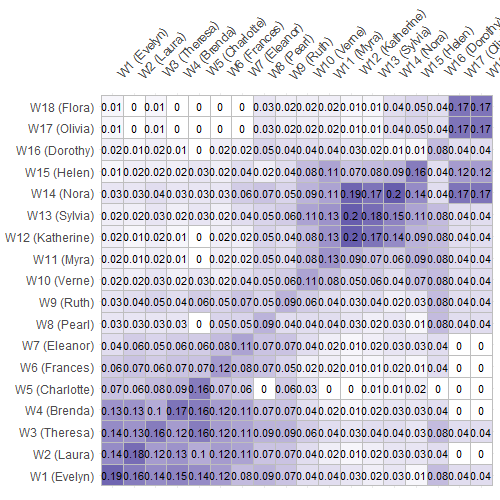
\includegraphics[width=1.0\textwidth]{Plots/p-norm.png}
            \caption{People.}
            \label{fig:p-dwproj}
    \end{subfigure} \\
     \begin{subfigure}[b]{0.55\textwidth}
        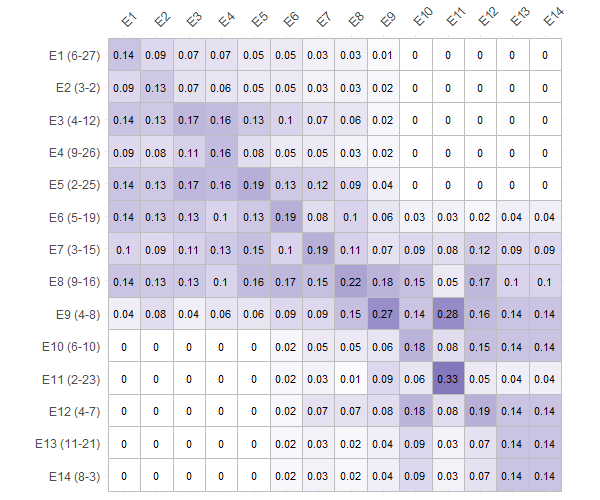
\includegraphics[width=1.0\textwidth]{Plots/g-norm.png}
            \caption{Groups.}
            \label{fig:g-dwproj}
    \end{subfigure}
    \caption{Degree-weighted projection matrices of the Southern Women data.}
    \label{fig:dwproj}
\end{figure}

It can be shown \citep{van2021correspondence}, that in the limit ($q \rightarrow \infty$), the iterative HH reflective scores can be obtained as a solution of the eigensystem:

\begin{equation}
    \mathbf{P}_{pp}C^R_p = \lambda_2C^R_p
    %\left(Dp^{-1}ADg^{-1}A^T\right)C^R_p = \lambda C^R_p
    \label{eq:dam1}
\end{equation}

\begin{equation}
    \mathbf{P}_{gg}C^R_g = \lambda_2C^R_g
    %\left(Dg^{-1}A^TDp^{-1}A\right)C^R_g = \lambda C^R_g
    \label{eq:dam2}
\end{equation}

With the $C^R$ scores for persons and groups obtained from the eigenvectors corresponding to the \textit{second} largest eigenvalue of the respective degree-weighted projection matrices, which are the same as the CA scores and the limit HH reflective scores \citep{van2021correspondence}.\footnote{As we have seen, both equations~\ref{eq:ca3} and~\ref{eq:ca4} produce row stochastic matrices; this means that their largest (dominant) eigenvalue will also be 1.0, which will be associated with a trivial first eigenvector containing constant values for both the people and the groups. Note also that the degree normalized projection matrices have equivalent sets of (non-zero) eigenvalues equal to the rank of the original affiliation matrix, with values between zero and one \citep{van2021correspondence}.} These scores will also be equivalent to the row and column scores corresponding to the first non-trivial dimension (for people and groups, respectively) obtained from a simple CA of the original affiliation matrix via SVD \citep[398, eq. 9.17]{fouss2016algorithms}. This exact correspondence can be verified in Figure~\ref{fig:ca-ref-corr}, which shows a scatterplot and associated linear regression line of the standardized scores computed via the iterative method of reflections ($q = 26$) on the y-axis against those obtained from the second eigenvector of the degree-weighted projection matrices for persons and groups on the x-axis ($r = 1.0$).\footnote{Formally, the eigendecomposition of the degree-weighted projection (for people) is given by the solution to the equation $\mathbf{P}_{pp} = \mathbf{UVU}^{-1}$, where $\mathbf{U}$ is a $|P| \times |P|$ matrix whose columns are the eigenvectors of $\mathbf{P}_{pp}$ and $\mathbf{V}$ is a $|P| \times |P|$ matrix whose diagonals are the eigenvalues of $\mathbf{P}_{pp}$ (with zeros in every other cell). Columns two through $|P|$ of matrix $\mathbf{U}$ contain the standard CA scores for the people along the complete set of $|P| - 1$ dimensions; the same goes for $\mathbf{P}_{gg}$ in the case of groups.}

Because $\mathbf{P}_{pp} = \mathbf{D}p^{-1}\mathbf{A}\mathbf{D}g^{-1}\mathbf{A}^T$ and $\mathbf{P}_{gg} = \mathbf{D}g^{-1}\mathbf{A}^T\mathbf{D}p^{-1}\mathbf{A}$ there is a formal equivalence in the duality relations implied by equations ~\ref{eq:dam1} and~\ref{eq:dam2} and that implied by the Bonacich two-mode centralities in equations~\ref{eq:bon3} and~\ref{eq:bon4}. Both extract individual and group scores as eigenvectors of the one-mode projection of the original affiliation matrix: $\mathbf{AA}^T$ and $\mathbf{P}_{pp}$ for people and $\mathbf{A}^T\mathbf{A}$ and $\mathbf{P}_{gg}$ for groups. The key difference is that in CA, we pre-multiply the affiliation matrix and its transpose by the inverse of the first-order centralities of the nodes in each mode before computing the eigenvalue decomposition, essentially normalizing the one-mode projection by the degrees of both sets of nodes. 

This can be clearly seen if we express $\mathbf{P}_{PP}= \mathbf{D}g^{-1}\mathbf{A}^T\mathbf{D}p^{-1}\mathbf{A}$ in terms of each cell entry \cite[eq. 4]{mealy2019interpreting}:

\begin{equation}
    p_{pp'} = \sum_g\frac{a_{pg}a_{p'g}}{C^R_p(1)C^R_g(1)} = 
    \frac{1}{C^R_p}\sum_g\frac{a_{pg}a_{p'g}}{C^R_g(1)}
    \label{eq:mealy1}
\end{equation}

In equation~\ref{eq:mealy1}, the numerator is equal to one when person $p$ and person $p'$ share membership in a group $g$. Summed across groups, this gives the number of memberships that $p$ and $p'$ have in common \citep{breiger1974duality}. As noted, the Bonacich dual centralities are obtained from the eigenvector corresponding to the first eigenvalue of this matrix of shared memberships (for people) and shared people (for groups). The HH reflective scores, on the other hand, are given by the eigenvectors of a weighted version of the same matrix, where the weights are the sizes of each of the groups $p$ shares with each other person summed across groups and divided by the total number of $p$'s memberships. 

The same reasoning applies to groups in the matrix $\mathbf{P}_{gg} = \mathbf{D}g^{-1}\mathbf{A}^T\mathbf{D}p^{-1}\mathbf{A}$, whose entries are given by:

\begin{equation}
    p_{gg'} = \sum_p\frac{a_{pg}a_{pg'}}{C^R_p(1)C^R_g(1)} = 
    \frac{1}{C^R_g}\sum_p\frac{a_{pg}a_{pg'}}{C^R_p(1)}
    \label{eq:mealy2}
\end{equation}

Now, as we saw earlier \citep[e.g.,][]{faust2005using} it turns out that this ``double-pre-weighting'' of each cell entry by the degrees of each mode (e.g., the row and column sums of the original affiliation matrix) is precisely that used for the CA of a two-mode matrix.\footnote{More accurately, cells are weighted by the inverse of the square root of the product of the row, and column sums \citep[e.g.,][124]{faust2005using}; accordingly, the first non-trivial CA dimension for persons and groups given by the right and left eigenvectors corresponding to the second-largest eigenvalue from the SVD of the matrix $\mathbf{D}_p^{-1/2}\mathbf{A}\mathbf{D}_g^{-1/2}$ \citep[126]{faust2005using}.} In fact, as \citet{mealy2019interpreting} have noted, the method of ``reflections'' is just a re-discovery of the older idea of computing CA scores via reciprocal averaging \citep{hill1973reciprocal}.

\begin{figure}
    \captionsetup[subfigure]{font=footnotesize,labelfont=footnotesize}
    \centering
     \begin{subfigure}[b]{0.45\textwidth}
        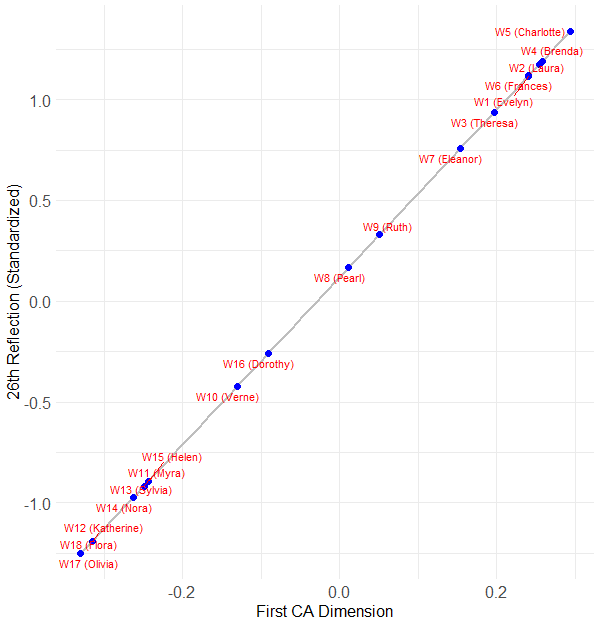
\includegraphics[width=1.0\textwidth]{Plots/p-ca-ref-corr.png}
            \caption{}
            \label{fig:p-ca-ref}
    \end{subfigure}
     \begin{subfigure}[b]{0.45\textwidth}
        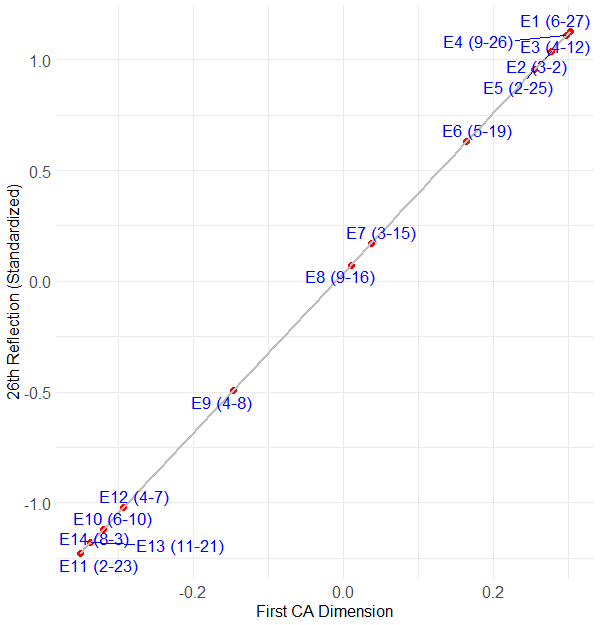
\includegraphics[width=1.0\textwidth]{Plots/g-ca-ref-corr.png}
            \caption{}
            \label{fig:g-ca-ref}
    \end{subfigure}
    \caption{Scatter plot of the scores computed by the method of reflections ($q = 26$) on the y-axis and the first dimension of the Correspondence Analysis of the two-mode affiliation matrix on the x-axis, for both persons (a) and groups (b). }
    \label{fig:ca-ref-corr}
\end{figure}

As \citet{desposito2014comparison} have recently noted, degree-pre-weighting does alter the original input data, which means that CA is \textit{not} meant to reproduce a low dimensional approximation of the original affiliation matrix. Indeed, it corresponds to moving from sums to averages, thus ``adjusting'' for the influence of person-activity and group size---a seemingly perennial issue in two-mode data analysis \citep[159ff]{bonacich1991simultaneous}. This can be seen by the fact that Equations~\ref{eq:mealy1} and~\ref{eq:mealy2} show that, substantively, what the degree pre-weighting does is that, for people, co-memberships count for more in determining interpersonal similarity when the group in question is small than when it is large, thus adjusting similarity by group size so that co-memberships in groups everyone belongs to counts for less \citep{ragozini2014correspondence}. In the same way, on the group side, shared members who do not have many affiliations count more in determining intergroup similarity than those with many affiliations. 

\begin{figure}[ht!]
    \captionsetup[subfigure]{font=footnotesize,labelfont=footnotesize}
    \centering
     \begin{subfigure}[b]{0.45\textwidth}
        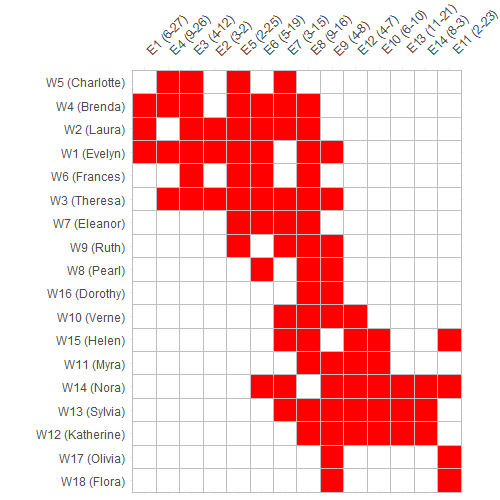
\includegraphics[width=1.0\textwidth]{Plots/ca-reord1.png}
            \caption{First CA Dimension}
            \label{fig:ca-reord1}
    \end{subfigure}
     \begin{subfigure}[b]{0.45\textwidth}
        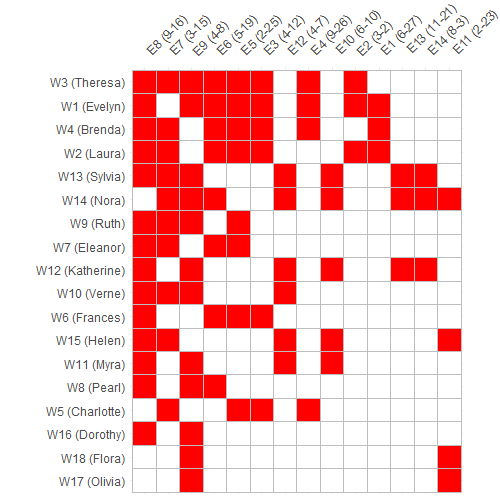
\includegraphics[width=1.0\textwidth]{Plots/bon-reord1.png}
            \caption{First Bonacich Dimension}
            \label{fig:bon-reord1}
    \end{subfigure}
     \begin{subfigure}[b]{0.45\textwidth}
        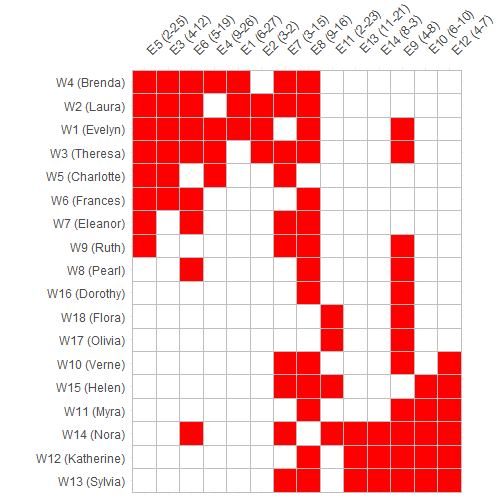
\includegraphics[width=1.0\textwidth]{Plots/bon-reord2.png}
            \caption{Second Bonacich Dimension}
            \label{fig:bon-reord2}
    \end{subfigure}
     \begin{subfigure}[b]{0.45\textwidth}
        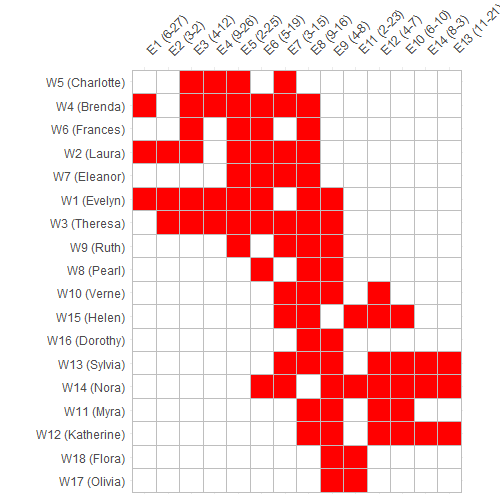
\includegraphics[width=1.0\textwidth]{Plots/SR-reord1.png}
            \caption{Second SimRank Eigenvector}
            \label{fig:sr-reord1}
    \end{subfigure}
    \caption{Southern Women Affiliation matrix with re-ordered rows and columns: (a) rows and columns re-ordered according to the person and group score on the first CA dimension, (b) rows and columns re-ordered according to person and group Eigenvector centrality score, (c) rows and columns re-ordered according to person and group score on the second Bonacich dimension, (d) rows and columns re-ordered according to the second eigenvector of the SimRank similarity matrix.}
    \label{fig:ca-v-bon}
\end{figure}

\section{Comparing Bonacich and CA Dual Scoring in the Southern Women Data} \label{sec:comparing}
\subsection{Row and Column Re-ordered Affiliation Matrices} 
Figures~\ref{fig:ca-reord1} and~\ref{fig:bon-reord1} illustrate the key differences between the two versions of dual two-mode scoring $C^R$ and $C^B$. Each panel shows the original Southern Women affiliation matrix but with rows and columns blocked according to the first CA dimension in (a) and the \citet{bonacich1991simultaneous} centrality in (b).\footnote{This, in effect, a two-mode version of constructing ``a posteriori'' (exploratory or data-driven) blockmodels, in the sense of \citet{wasserman1987stochastic}, using scores from CA and Bonacich scoring to re-order the original matrix, as they did in that paper for one-mode networks.} In the plot, a cell entry is colored red if it has a one in the original affiliation matrix and is white when the corresponding entry is zero. As we can see, the two row-column-reshuffled matrices have appreciably distinct structures, with the $C^R$ re-ordered affiliation matrix having a block-diagonal structure \citep[34]{wasserman1990correspondence}, and the $C^B$ re-ordered affiliation matrix having a triangular structure. 

Accordingly, the $C^R$ reflective scores reveal a dual-block partition between groups of women who selectively attend two groups of events (on the top-right and bottom-left of the plot). The traditional eigenvector centrality re-ordering, on the other hand, reveals a classic \textit{core-periphery} partitioning \citep{borgatti2000models}, with a group of highly active women (on the top half) who selectively co-participate in highly attended events (on the left-hand side) and less active women (on the bottom half) who go to less well-attended events (on the right-hand side). In fact, as \citet[p. 206]{everett2013dual} have noted, computing the eigenvector scores for both sets of nodes in the mode network from the classic \citet{breiger1974duality} projections---as in \citet{bonacich1991simultaneous}---and using them to re-order the rows and columns of the original affiliation matrix is a way to approximate using continuous scores an ideal discrete core-periphery partitioning of the two-mode data matrix, cheaper and more efficiently compared to discrete optimization methods. In fact, the two-block core-periphery partitioning of people and groups suggested by Figure~\ref{fig:bon-reord1}---separating the first eight women starting from the top from the rest and the first five events starting from the left from the rest) is substantively identical to that shown in~\citet[206, Table 2]{everett2013dual}, who previously extracted a core-periphery partitioning of the same data.

\begin{figure}[ht!]
    \centering
        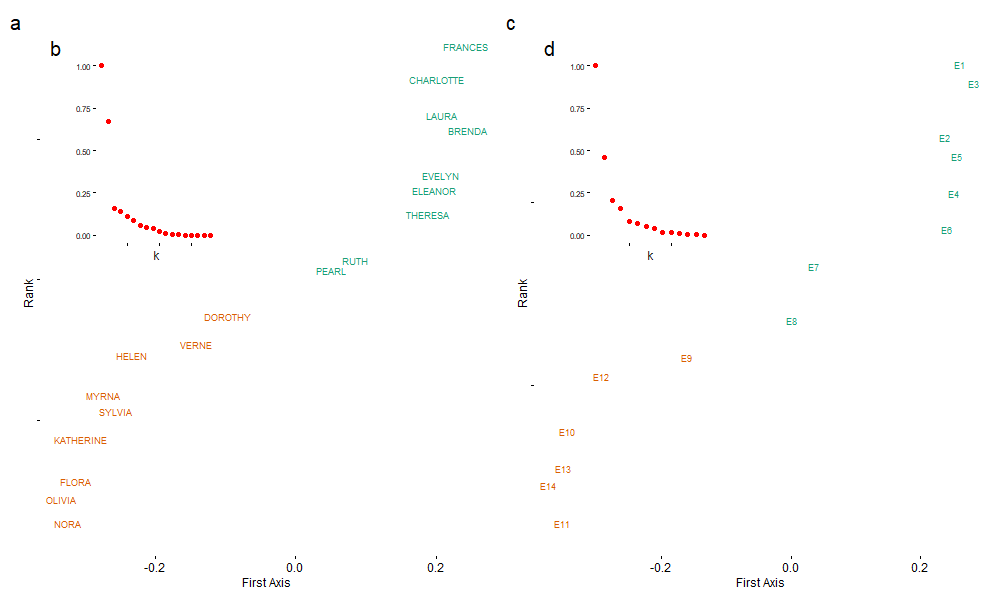
\includegraphics[width=0.8\textwidth]{Plots/ca-eigvec.png}            
        \label{fig:eigvec}
    \caption{CA Eigenvector plot for persons (a) and groups (b). The first dimension CA score is on the x-axis, and the rank order of persons and groups on the same score is on the y-axis. The inset plot (c) shows the eigenvalue orderings on the x-axis ($k$) for persons and groups, showing a separation between the first three eigenvalues and the rest.}
    \label{fig:ca-eigvec}
\end{figure}

\subsection{Eigenvector Plot} \label{subsec:eigplot}
We can confirm that the first CA axis points toward the underlying similarity-based partitioning of the two-mode network by looking at Figure~\ref{fig:ca-eigvec}(a) and~\ref{fig:ca-eigvec}(c), which shows the $C^R$ score of persons and groups on the x-axis against the score's rank order on the y-axis. If a two-mode network has no discernible block structure, the first dimension CA scores would be distributed as a continuous logistic curve; when block structure is present, we should observe discernible breaks in this distribution \citep{van2021correspondence}. The Southern Women Data clearly belong in the second category. In the people mode, we have \{Frances, Laura, Brenda, Charlotte, Evenly, Theresa, Elanor, Ruth, Pearl\} on one side, \{Dorothy, Nora, Katherine, Sylvia, Flora, Olivia, Myra, Helen, Verne\} on the other. Among events, we have \{E1, E2, E3, E4, E5, E6\} on side \{E9, E10, E11, E12, E13, E14\} on the other and \{E7, E8\} in an ambiguous middle position. Note that this is the canonical consensus partitioning (for the people) highlighted by \citet{freeman2003finding} across twenty-one different methods and subsequently reproduced (for both persons and groups) by \citet{kovacs2010generalized} and \citet{lizardo2024two} using a generalized relational similarity (GRS) approach. This indicates that persons and groups receive similar scores in the first dimension of CA only when they have similar connectivity similar to \textit{similar} groups, where group similarity is defined dually as having members in common who are themselves similar; we will return to this point in Section~\ref{sec:cagensim}. 

\begin{figure}[ht!]
    \captionsetup[subfigure]{font=footnotesize,labelfont=footnotesize}
    \centering
        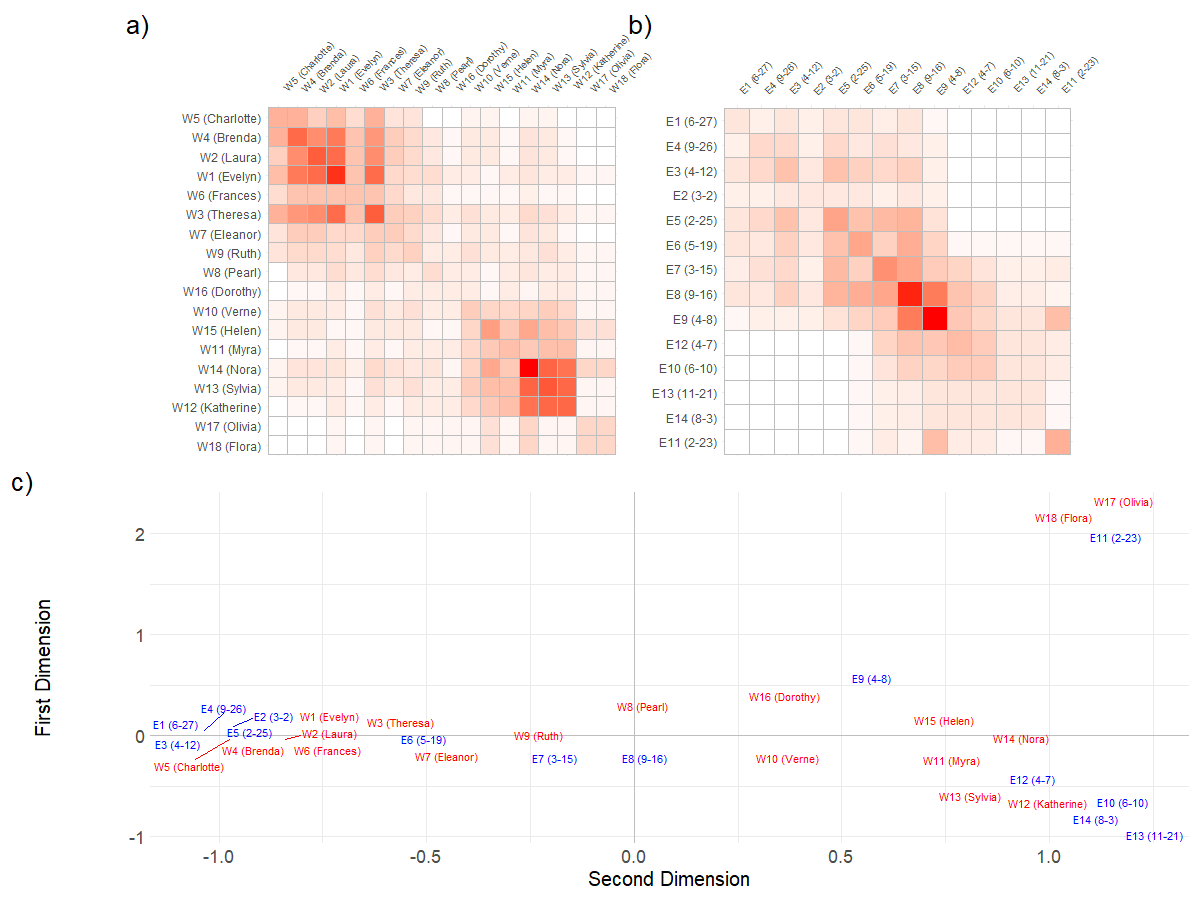
\includegraphics[width=1.0\textwidth]{Plots/ca-corr-plot.png}
    \caption{The top panels show the degree-weighted one-mode projection heatmap plots for (a) persons and (b) groups in the Southern Women Data with rows and columns re-ordered according to the first CA dimension. Darker red cells correspond to high entry values (normalized by the maximum) in the $\mathbf{P}_{pp}$ and $\mathbf{P}_{gg}$ matrices. The bottom panels show the correspondence plot for persons and groups with scores corresponding to (c) the first dimension on the horizontal axis with the second dimension on the vertical axis, and (d) the first dimension on the horizontal axis with the third dimension on the vertical axis.}
    \label{fig:ca}
\end{figure}

\subsection{Degree-Weighted Projections and CA Correspondence Plot} \label{subsec:caplot}
Panels (a) and (b) of Figure~\ref{fig:ca} shows a heatmap plot of the same weighted projection matrices from Figures~\ref{fig:p-dwproj} and~\ref{fig:g-dwproj}, but this time with the rows and columns re-ordered according to the scores corresponding to the first CA dimension. In the plot, darker red indicates greater similarity between pairs of persons and groups, and gray indicates less similarity. The bottom panels of the same figure show the usual correspondence plot of the first three CA dimensions, with the first dimension on the x-axis against the second dimension on the y-axis in panel (c) and the first dimension plotted against the third dimension on the y-axis in panel (d). 

This figure illustrates several important points. First, as the heatmap plots in panels (a) and (b) show, distances along the first CA axis correspond to degree-weighted similarities between persons and groups recorded in the $\mathbf{P}_{pp}$ and $\mathbf{P}_{gg}$ matrices. Pairs of people and groups with the largest entries in the matrix have minimal differences in the first CA dimension score, appearing close to one another when we reshuffle the rows and columns of the weighted projection matrix. This also means that the distances between pairs of people and groups in the standard correspondence plot---usually taken to be a low-dimensional representation of the \textit{original} affiliation matrix \citep{borgatti1997network}---are best thought of as low-dimensional representations of the respective \textit{degree-normalized one-mode projections}. Pairs of people with large values in the projection matrix $P_{pp}$---such as \{Olivia, Flora\},  \{Katherine, Sylvia, Nora\}, \{Dorothy, Verne\}, and \{Brenda, Laura, Evelyn\}--- appear closer in the correspondence plot. The same goes for pairs of groups; those with large values in $P_{gg}$ matrix---such as \{E13, E14\} and \{E1, E2, E3, E4\}---appear closer in the correspondence plot, while those with small weighted similarity values are placed far apart. Distances between same-mode entities in the correspondence plot are thus a function of their (inverse) degree-normalized similarity.

Note that this differs from the usual interpretation of the CA correspondence plot, which is typically taken to bring together nodes with ``similar'' connectivity patterns, where similarity is presumed to be a function of their raw row profiles (for people) or column profiles (for groups), a criterion closer to structural equivalence~\citep{desposito2014comparison}, or ``first order'' similarity \citep{kovacs2010generalized}. This interpretation implies (for instance) that two people who attend many of the same events or groups with many members in common will appear close in the plot. But this (still common) interpretation is off the mark. What the CA correspondence plot distance captures is, instead, people and groups that are \textit{surprisingly} similar (e.g., from the point of view of a suitable null model, like independence) after taking people's activity levels and the sizes of the groups they belong to into account. This type of degree-normalization can be the preferred approach in some applications since people with many memberships and groups with many members will appear to be similar to many other people and groups if we go with the raw number of other-mode objects shared.\footnote{Note that this, finding ``surprising'' similarities in terms of the indirect paths linking nodes in a network after the main effects of node-connectivity are considered, is the same rationale given by \cite{leicht2006vertex} for weighting the \citet{katz1953new} similarity matrix by the degrees of the corresponding nodes \citep[see][68, eqs. 2.13 and 2.14]{fouss2016algorithms}. As we have seen, this is precisely the key contrast between the Bonacich and the CA dual centrality measures for two-mode networks.} This implies that the similarities between pairs of people and groups will be weighted by the degrees of the other-mode objects that are shared between them. Thus, people who share memberships in small groups will be closer in the diagram than people who share memberships in big groups. In the same way, groups that share people with few memberships will be closer in the diagram than those sharing people with many other memberships \citep{desposito2014comparison}. 

Another thing to note is that since the CA row and column scores in each dimension are obtained from the eigendecomposition and subsequent low-rank approximation of the degree-normalized similarity matrices $\mathbf{P}_{pp}$ and $\mathbf{P}_{gg}$, each dimension provides independent information on the similarity clustering of persons and groups.\footnote{We know from inset plot (c) of Figure~\ref{fig:ca-eigvec} that the eigenvalues corresponding to the first three dimensions exhibit strong separation from the rest, suggesting that these provide a good low-rank approximation of the original degree-weighted projection matrix for persons and groups.}  Thus, as shown in panels (c) and (d) of Figure~\ref{fig:ca}, as we have already seen, the first horizontal dimension recovers the main partition separating the two dominant clusters of persons and groups~\citep{freeman2003finding}. The second and third dimensions, by contrast, recover secondary and tertiary similarity clusters of people and groups independent of the main two-block partition. Thus, the second dimension (the y-axis in panel (c) of Figure~\ref{fig:ca}) separates \{Flora, Nora\} and \{E9, E11\} from the rest of persons and groups, consistent with the strong similarity between these nodes in the original weighted projection matrix. We know from the original affiliation matrix in Figure~\ref{fig:sw} that \{Flora, Nora\} are maximally similar---they are structurally equivalent---and \textit{only} attend events \{E9, E11\}, which makes these events similar in the second dimension given they are attended by the two people who are also most similar in the same dimension (this also accounts for the high similarity between the two events shown in the heatmap plot of the degree-weighted projection in Figure~\ref{fig:ca}(b)). 

The third CA dimension, shown in the y-axis in panel (d) of Figure~\ref{fig:ca} against the first dimension separation on the x-axis, by contrast, separates \{Eleanor, Pearl, Ruth, Dorothy, Verne, Myra\} and \{E8, E9\} from the rest. We know from Figure~\ref{fig:bon-reord1} that event E8, along with E7, is one of the most popularly attended events and thus contributes little to differentiate between the main partition of people and events on the first correspondence plot in panel (c), hence its location near the plot's origin. The pattern of attendance of these six women is one characterized by affiliation with these popular events combined with sparser attendance at the events that most serve to differentiate the two primary clusters. In his original paper, \citet[164]{bonacich1991simultaneous} noted that this third dimension ``corresponded closely to the centrality analysis pattern,'' an observation likely driven by the affinity between the actors who load highly on this dimension and two of the most central events by raw popularity, \{E8, E9\}. What we can see instead is that the third CA dimension separates actors that are most ``peripheral'' to the two main clusters according to \citet{freeman2003finding}; namely, \{Eleanor, Pearl Ruth\} on one side and \{Dorothy, Verne, Myra\} on the other, from core members of the two main blocks, who are placed in the bottom of the correspondence plot in panel (c)---low scores in the third dimension---and toward the extreme left and right ends of the plot, indicating very high absolute value scores in the first dimension. 

\subsection{Breiger Projections and the Bonacich Correspondence Plot} \label{sec:eigplot}
Earlier, we discussed how CA is sometimes considered a technique useful to generate a correspondence plot that provides a ``low-dimensional approximation to the input data'' \citep[125]{faust2005using}, where the ``input data'' is presumed to be the original affiliation matrix $\mathbf{A}$. But as we have seen, this is \textit{not} what CA is designed to do. Instead, CA is meant to provide a low-dimensional approximation of a \textit{transformed} version of the input data, where the transformation is meant to adjust for people's activity levels and group sizes \citep{desposito2014comparison}. In fact, CA is better thought of as a low-dimensional approximation of the degree-weighted projection of the affiliation matrix, as given by equations~\ref{eq:dam1} and~\ref{eq:dam2}, which represents a degree-adjusted proximity matrix---or a Markov transition matrix under a different interpretation---between pairs of people and pairs of groups after accounting for their respective activity and sizes, respectively.

Here, once again, the contrast with the traditional dual Bonacich scores can prove instructive. Figures~\ref{fig:bon-sim}(a) and~\ref{fig:bon-sim}(b) shows the ``raw'' (unweighted by degree) similarity scores for persons ($a_{pp'} = \sum_g a_{pg}a_{p'g}$) and groups ($a_{gg'} = \sum_p a_{pg}a_{pg'}$)---the standard \citet{breiger1974duality} projections---with the rows and columns re-ordered according by the first eigenvector of the matrix, which is equivalent to the usual Bonacich eigenvector dual centrality score for two-mode networks (see equations~\ref{eq:bon3} and~\ref{eq:bon4}). Both similarity matrices reproduce the triangular, core-periphery structure we observed in the re-ordered affiliation matrix in Figure~\ref{fig:ca-v-bon}(b). Figure~\ref{fig:bon-sim}(c) plots $C^B$ on the x-axis against the second eigenvector of the unweighted similarity matrix. 

This suggests that the eigenvector centralities do encode a kind of similarity between pairs of people and pairs of groups; it just happens to be based on the unweighted similarity scores given by the raw number of shared memberships (for people) and shared members (for groups). In this respect, the dual centrality eigenvector score mixes an ordinal rank criterion with a similarity criterion since people with lots of memberships will end up being ``similar`` to more people on the standard projection matrix by the simple fact of having more memberships (and the same for large groups with respect to members). Persons and groups high in eigenvector centrality can be thought of as being the most similar to most others, condensing the information in the Breiger projection matrix into a single ordinal rank. Also, just like with CA and the degree-weighted projections, higher-order axes of the Bonacich centrality eigendecomposition of the Breiger projection matrices should also encode forms of similarity between pairs of people and pairs of groups, net of the main axis dominated by overall person activity and group size.  

\begin{figure}[ht!]
    \captionsetup[subfigure]{font=footnotesize,labelfont=footnotesize}
    \centering
        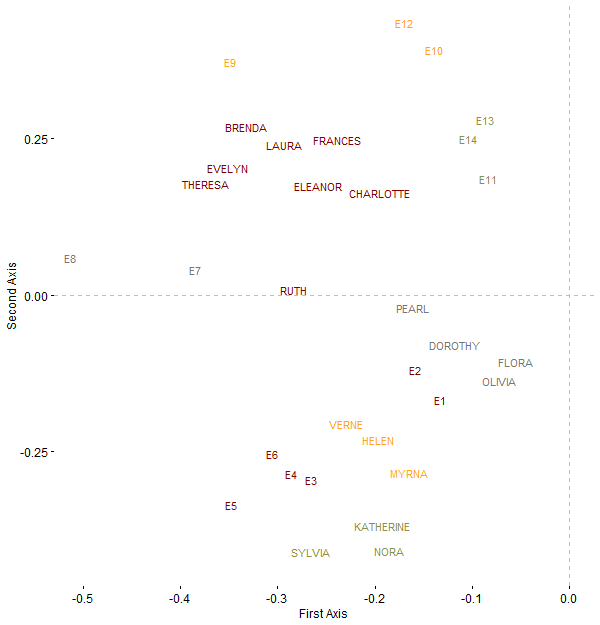
\includegraphics[width=1.0\textwidth]{Plots/bon-corr-plot.png}
            \caption{Bonacich correspondence plot.}
            \label{fig:bon-corr}
    \caption{Bonacich dual centrality similarity plots for persons (a) and groups (b) on the left and right top panel. The bottom panel (c) shows the Bonacich eigenvector centrality correspondence plot for persons and groups with scores corresponding to the standard Bonacich eigenvector centrality on the horizontal axis and scores corresponding to the second largest eigenvector of the affiliation matrix on the vertical axis, points are colored according a k-means three-cluster solution.}
    \label{fig:bon-sim}
\end{figure}

While plotting the Bonacich centrality against higher eigenvectors is not necessarily a substantively unmotivated practice \citep[see][for discussion in the one-mode network case]{iacobucci2017eigenvector} the exact meaning of the mysterious second eigenvector remains unclear in the two-mode case. We can use the same ``a posteriori blockmodeling'' approach we used before to contrast CA and the Bonacich centrality analysis to shed light on this issue \citep{wasserman1987stochastic}. Figure~\ref{fig:bon-reord2} shows the affiliation matrix blocked according to the \textit{second} Bonacich dimension, and Figure~\ref{fig:bon-sim} (c) shows the ``Bonacich Correspondence Plot'' with the usual eigenvector centrality score on the horizontal x-axis plotted against the second eigenvector of the Breiger projection matrix for both persons and groups on the vertical y-axis. 

We can see from Figure~\ref{fig:bon-reord2} that the second Bonacich dimension diplays a \textit{dual triangular} structure, revealing two secondary core and peripheries not evident in the blocking according to either the first CA or standard eigenvector scores. Interestingly, this partition is almost equivalent to that obtained in \citet[Table 5]{everett2013dual} by clustering a version of the projection matrices of the Southern Women data where the proximities were designed to detect \textit{structural equivalence}.\footnote{In that application, the cell entry in each projection matrix was the \textit{proportion of matches} between each pair of people and groups. As \citet[208]{everett2013dual} define it, ``[p]roportion matching is the number of times two profiles have the same entry (either zeros or ones) divided by the length of the profile.''} In Everett and Borgatti's \citeyearpar[208]{everett2013dual} clustering solution, ``[t]he women are then split into (a) those that attend four or fewer events and consequently attend very few of the peripheral events (Pearl, Ruth, Verne, Myrna [sic], Dorothy, Olivia, Flora), and (b) those that attend core events and the first group of peripheral events (Evelyn, Laura, Theresa, Brenda, Charlotte, Francis, Eleanor), and (c) those that attend core events and the second group of peripheral events (Helen, Katherine, Sylvia, Nora).'' Note that the only disagreement between Everett and Borgatti's partition and the three-block solution suggested by Figure~\ref{fig:bon-reord2} is Myrna/Myra's position, who is assigned to Borgatti and Everett's third group in the a posteriori blocking obtained from Bonacich's second dimension. This may be partly due to the discrepant position of ``core event'' E9 along the columns of the blocked matrix which is grouped with the second group of ``peripheral'' events \{E10, E11, E12, E13, E14\} in Figure~\ref{fig:bon-reord2}. 

This analysis points to a new way to interpret the second Bonacich dimension, namely, as a way to reveal secondary core-periphery partitions net of a main core-periphery partition in the two-mode network (if any exists). Furthermore, the similarities between persons and groups defined over the two-dimensional Bonacich space, shown in Figure~\ref{fig:bon-sim} (c), can thus be used to reveal \textit{structurally equivalent} clusters of persons and events similar to those obtained by \citet[Table 5]{everett2013dual}. This is confirmed by the coloring of the persons and groups in Figure~\ref{fig:bon-reord2}) which comes from a k-means cluster analysis using the first two Bonacich dimensions to define initial cluster centroids, revealing a three-cluster solution almost equivalent to that obtained by Everett and Borgatti, with the exception of Myrna/Myra's and event E9's assingment as discussed earlier. This suggests that the Bonacich approach to similarity clustering is distinct from CA in being useful for revealing structural equivalence, thus making the Bonacich dimensions a more faithful basis for a low-rank reconstruction of the original ``input data'' than CA if that is the goal of the analysis \citep{desposito2014comparison}. 

\section{Correspondence Analysis and Generalized Relational Similarity} \label{sec:cagensim}
As noted, there seems to be a relationship between the ordering of persons and groups produced by CA of a two-mode network and that produced by previous work using a ``generalized relational similarity'' (GRS) strategy. Recall that for objects (let us say people) to be similar according to the GRS criterion, they must have overlapping connections, and those links should go to objects in the other mode \textit{that are themselves similar}, where objects' similarities are given by their pattern of connections to objects in the other mode. This recursive definition of similarity thus recalls the classic distinction between structural and regular equivalence \citep{everett1994regular}. In the context of two-mode networks, \citet{kovacs2010generalized} proposed one such approach to defining a GRS for nodes in one and two-mode networks using a modified version of the correlation distance.\footnote{\citet{lizardo2024two} shows the connection between Kovacs's idea of generalized relations similarity and the two-mode network projection.}

An earlier effort to define a GRS for persons and groups in two-mode networks, one more relevant for a direct comparison with CA and the ``reflective'' approaches already considered, can be found in \citet{jeh2002simrank}. In that work, the authors dubbed their similarity measure ``SimRank.'' In the context of two-mode network analysis, the goal is to compute a matrix of similarities for each of the two-node sets, where the similarity of people is a function of the groups they belong to, and the similarity of groups is a function of the people who belong to them, making the similarity of persons and groups ``mutually reinforcing notions'' \citep[540]{jeh2002simrank}. Thus,

\begin{itemize}
    \item People are \textit{similar} if they belong to \textit{similar} groups.
    \item Groups are \textit{similar} if they share \textit{similar} members.
\end{itemize}

This definition consistent with a GRS approach \citep[see][]{kovacs2010generalized, lizardo2024two}. To accomplish this, \citet[540, eq. 2 and eq. 3]{jeh2002simrank} propose that we define the similarity of each pair of people $S(p, p')$  as given by:

\begin{equation}
    S(p, p') = \frac{\alpha}{C^R(1)_pC^R(1)_{p'}}
    \sum_{i = 1}^{C^R(1)_p} \sum_{j = 1}^{C^R(1)_{p'}} 
    S\left(g(i)_{i \in N(p)}, g(j)_{j \in N(p')}\right)
    \label{eq:simrank1}
\end{equation}

Where everything is as before, and $g(i)_{i \in N(p)}$ is the $i^{th}$ group in the set of groups that person $p$ belongs to, $g(j)_{j \in N(p')}$ is the $j^{th}$ group in the set of groups that person $p'$ belongs to, and $\alpha$ is a free parameter obeying the restriction: $0 > \alpha < 1$. By construction, $S(p, p) = 1$, for all $p$. Thus, equation \ref{eq:simrank1} says that the SimRank similarity between two people is a function of the sum of the similarities of each unordered pair of groups they both belong to, weighted by the reciprocal of the products of their number of memberships multiplied by $\alpha$.

Likewise, for groups, the SimRank similarities are given by:

\begin{equation}
    S(g, g') = \frac{\alpha}{C^R(1)_gC^R(1)_{g'}}
    \sum_{i = 1}^{C^R(1)_g} \sum_{j = 1}^{C^R(1)_{g'}} 
    S\left(p(i)_{i \in N(g)}, p(j)_{j \in N(g')}\right)
    \label{eq:simrank2}
\end{equation}

Where $p(i)_{i \in N(g)}$ is the $i^{th}$ person in the set of members of group $g$, and $p(j)_{j \in N(g')}$ is the $j^{th}$ person in the set of members of group $g'$, and $S(g, g) = 1$. Thus, the SimRank similarity between two groups is a function of the sum of the similarities of each pair of people who belong to both groups, weighted by the reciprocal of the products of the number of members of each group multiplied by $\alpha$.

\begin{figure}
    \captionsetup[subfigure]{font=footnotesize,labelfont=footnotesize}
    \centering
        
\includegraphics[width=0.9\textwidth]{Plots/simrank-v-ca.png}
            \label{fig:sim-v-ca}
    \caption{Simrank versus CA comparison. Panels (a) and (c) show the final SimRank similarity matrices for persons and groups (respectively) with rows and columns ordered according to the first CA dimension scores.  Panel (b) shows the Pearson correlation between the scores corresponding to the second eigenvector of the SimRank similarity matrix (on the y-axis) and the scores corresponding to the first CA dimension (on the x-axis) for persons, panel (d) shows the same correlation for groups.}
    \label{fig:simrank}
\end{figure}

In two-mode networks, SimRank scores for each pair of nodes across the two sets can be estimated via a simple algorithm, in which we first estimate $S(p, p')$ in equation \ref{eq:simrank1} using baseline values. Hence, only groups that two people share contribute to the initial values of $S(p, p')$ since only $S(g, g)>0$ at the outset. We then plug those values into equation \ref{eq:simrank2}, then loop back to equation \ref{eq:simrank1} with the resulting $S(g, g')$ values, and continue iterating until convergence---generally achieved after five iterations \citep{jeh2002simrank}, which is confirmed here for the Southern Women data. 

Note that equations~\ref{eq:simrank1} and~\ref{eq:simrank2} share a formal similarity with HH's ``method of reflections'' discussed earlier, in particular, the fact that both compute quantities based on nodes in the other mode averaged by the degree of nodes in the focal mode. The key difference is that SimRank works directly with pairwise comparisons between node dyads \citep{jeh2002simrank}. Nevertheless, this double weighting by degree should make us suspect that the results of the SimRank similarity analysis would not be too far from those obtained via CA, given the mathematical equivalence of CA and the method of reflections \citep{mealy2019interpreting, van2021correspondence}. Beyond that, the SimRank approach can be thought of as yet another way of obtaining one-mode projections from an original two-mode network, in line with Everett and Borgatti's ``dual projection'' approach \citep{everett2013dual}.

Figure~\ref{fig:sr-reord1} shows the original affiliation matrix, this time with rows and columns re-arranged according to the values of the main non-trivial eigenvector (corresponding to the second-largest eigenvalue) of the SimRank similarity matrices---with $\alpha$ set to $0.8$---for the row and column nodes. Like in Figure~\ref{fig:ca-v-bon}(a), this reshuffling displays a block-diagonal structure separating the two communities of persons and groups as that revealed by CA, suggesting that CA and SimRank uncover a similar underlying partitioning of the two-mode network's community structure. Figure~\ref{fig:simrank-v-ca}(a) and Figure~\ref{fig:simrank-v-ca}(b) show an eigenvector plot similar to that shown in Figures~\ref{fig:ca-eigvec}(a) and Figure~\ref{fig:ca-eigvec}(b) but this time with the main eigenvector of SimRank similarity matrices of both persons and groups on the x-axis and the corresponding rank on the y-axis. Looking at the plots from left to right, we can see that the partitioning of the node sets on the most informative eigenvector of the SimRank similarity matrix is substantively equivalent to those revealed by the first CA eigenvector, separating similar blocks of people and events. Figures~\ref{fig:simrank-v-ca}(c) and (d) show a regression plot of the first CA dimension scores for persons and groups (respectively) on the x-axis and the SimRank scores extracted from the main non-trivial eigenvector of the SimRank similarity matrix for both persons and groups on the y-axis. As we can see, the CA and SimRank ordering of nodes along the first dimension agree quite closely ($r = 0.98$ for persons and $r = 0.99$ for groups), confirming that these first eigenvectors capture the same (GSR) information across the two approaches. 

\section{Discussion and Concluding Remarks} \label{sec:disc}
This paper reconsiders the role of CA in the analysis of two-mode network data. We began with an accidental ``rediscovery'' of CA in the analysis of two-mode networks via a ``reflective'' approach \citep{hidalgo2009building}, showing that the method of reflections leads to an eigenvector-style solution that is equivalent to simple CA of the affiliation matrix. Working backward from this, we also clarified the linkages between CA and the more commonly used eigenvector approach for calculating dual centralities in two-mode data due to \citet{bonacich1991simultaneous}. I showed that just like the reflective scores that converge to the CA scores of the affiliation matrix, we could also think of the Bonacich centralities as the equilibrium solution to reflective iterations through the two-mode matrix, with the main difference being that the CA reflections deal with sums of averages weighted by the degrees of nodes in each mode, while the Bonacich approach works with unweighted (but normalized) sums. This exercise clarifies the links between CA and the dual two-mode eigenvector centrality more coherently and systematically, an issue that was left open and somewhat unclear in Bonacich's \citeyearpar{bonacich1991simultaneous} classic paper. Thus, one conclusion that emerges from this analysis is that CA computes a kind of centrality for two-mode networks, equivalent to Hidalgo and Hausman's ``reflective'' centrality \citep{van2021correspondence}.

But CA does more than reveal a latent dual ordering of nodes in the two-mode network. In addition to doing this, CA can be shown to reveal \textit{groupings} of nodes based on some conception of the similarity of their connections to nodes in the other mode. This is evident once we use the scores of the first CA dimension to re-order the rows and columns of the original affiliation matrix. When the CA scores are used, a clear (and now well-known) dual partition between persons and groups emerges in the classic Southern Women data. This partition is substantively distinct from that which would emerge if we use the same approach to re-ordering the original data using the Bonacich centralities, which instead uncover a latent core-periphery partition between actors and events \citep{everett2013dual}. 

This is another way in which CA and the Bonacich dual centrality approach systematically differ; one is geared to uncovering blocks of actors with similar connections to events in the other mode (and vice versa), while the other reveals blocks of actors who are the most active and who attend the largest events. Both are, of course, legitimate ways of analyzing the structure of a two-mode network. Still, they differ in terms of the structural patterns that they are sensitive to, with the CA approach closer to a community partition where nodes that are surprisingly similar end up in the same clusters---where ``surprising'' means similarity based on deviations from a suitable null model based on random mixing given their first-order degrees. 

But what kind of similarity is the clustering based on the CA of the two-mode network sensitive to? Here, we show that CA recovers a type of generalized relational similarity (GRS). That is, actors who have similar patterns of linkage to similar events are deemed similar, while events that have similar patterns of connectivity to similar actors are also deemed similar. Using a well-known iterative method to recover such generalized similarities from two-mode networks \citep{jeh2002simrank}, we saw that the scores from the first dimension of CA end up being a fairly accurate approximation to the resulting partition from the generalized relational similarity approach. Thus, we can clarify that two-mode network CA reveals latent groupings of nodes based on a GRS criterion. 

Overall, the preceding has shown that CA can be upgraded from a method designed to generate joint plots and visualization of two-mode data to one that can be seen as more ``central'' to the usual social-network-analytic tasks, like ordering the nodes in the two sets according to some substantively meaningful rank---centrality analysis---or finding sets of similar actors in the network (subgroup or community detection). At the very least, it seems like the Bonacich style dual centrality based on the eigenvector decomposition of the raw affiliation matrix should not be the default ``reflective'' centrality approach unless the analyst has the explicit analytic goal of exploring center-periphery partitioning in the network. 

A better approach, similar to the one exemplified here, would be to present a comparison of the reflective scores obtained by CA and Bonacich side-by-side to see whether the underlying display a substantively interesting similarity partitioning in addition to any core-periphery ordering. Of course, suppose the analyst is more interested in such a ``subgroup'' analytic approach. In that case, the Bonacich dual centrality approach is less helpful (even if multiple dimensions are considered), and CA should be the first line of attack. 



%% Loading bibliography style file]
%\bibliographystyle{model1-num-names}
\bibliographystyle{cas-model2-names}
% Loading bibliography database
\bibliography{ca.bib}
\end{document}


The Elsevier cas-dc class is based on the
standard article class and supports almost all of the functionality of
that class. In addition, it features commands and options to format the
\begin{itemize} \item document style \item baselineskip \item front
matter \item keywords and MSC codes \item theorems, definitions and
proofs \item labels of enumerations \item citation style and labeling.
\end{itemize}

This class depends on the following packages
for its proper functioning:

\begin{enumerate}
\itemsep=0pt
\item {natbib.sty} for citation processing;
\item {geometry.sty} for margin settings;
\item {fleqn.clo} for left aligned equations;
\item {graphicx.sty} for graphics inclusion;
\item {hyperref.sty} optional packages if hyperlinking is
  required in the document;
\end{enumerate}  

All the above packages are part of any
standard \LaTeX{} installation.
Therefore, the users need not be
bothered about downloading any extra packages.

\section{Installation}

The package is available at author resources page at Elsevier
(\url{http://www.elsevier.com/locate/latex}).
The class may be moved or copied to a place, usually,\linebreak
\verb+$TEXMF/tex/latex/elsevier/+, %$%%%%%%%%%%%%%%%%%%%%%%%%%%%%
or a folder which will be read                   
by \LaTeX{} during document compilation.  The \TeX{} file
database needs updation after moving/copying class file.  Usually,
we use commands like \verb+mktexlsr+ or \verb+texhash+ depending
upon the distribution and operating system.

\section{Front matter}

The author names and affiliations could be formatted in two ways:
\begin{enumerate}[(1)]
\item Group the authors per affiliation.
\item Use footnotes to indicate the affiliations.
\end{enumerate}
See the front matter of this document for examples. 
You are recommended to conform your choice to the journal you 
are submitting to.

\section{Bibliography styles}

There are various bibliography styles available. You can select the
style of your choice in the preamble of this document. These styles are
Elsevier styles based on standard styles like Harvard and Vancouver.
Please use Bib\TeX\ to generate your bibliography and include DOIs
whenever available.

Here are two sample references: 
\cite{Fortunato2010}
\cite{Fortunato2010,NewmanGirvan2004}
\cite{Fortunato2010,Vehlowetal2013}

\section{Floats}
{Figures} may be included using the command,\linebreak 
\verb+\includegraphics+ in
combination with or without its several options to further control
graphic. \verb+\includegraphics+ is provided by {graphic[s,x].sty}
which is part of any standard \LaTeX{} distribution.
{graphicx.sty} is loaded by default. \LaTeX{} accepts figures in
the postscript format while pdf\LaTeX{} accepts {*.pdf},
{*.mps} (metapost), {*.jpg} and {*.png} formats. 
pdf\LaTeX{} does not accept graphic files in the postscript format. 

\begin{figure}
	\centering
		\includegraphics[scale=.75]{figs/Fig1.pdf}
	\caption{The evanescent light - $1S$ quadrupole coupling
	($g_{1,l}$) scaled to the bulk exciton-photon coupling
	($g_{1,2}$). The size parameter $kr_{0}$ is denoted as $x$ and
	the \PMS is placed directly on the cuprous oxide sample ($\delta
	r=0$, See also Table \protect\ref{tbl1}).}
	\label{FIG:1}
\end{figure}


The \verb+table+ environment is handy for marking up tabular
material. If users want to use {multirow.sty},
{array.sty}, etc., to fine control/enhance the tables, they
are welcome to load any package of their choice and
{cas-dc.cls} will work in combination with all loaded
packages.

\begin{table}[width=.9\linewidth,cols=4,pos=h]
\caption{This is a test caption. This is a test caption. This is a test
caption. This is a test caption.}\label{tbl1}
\begin{tabular*}{\tblwidth}{@{} LLLL@{} }
\toprule
Col 1 & Col 2 & Col 3 & Col4\\
\midrule
12345 & 12345 & 123 & 12345 \\
12345 & 12345 & 123 & 12345 \\
12345 & 12345 & 123 & 12345 \\
12345 & 12345 & 123 & 12345 \\
12345 & 12345 & 123 & 12345 \\
\bottomrule
\end{tabular*}
\end{table}

\section[Theorem and ...]{Theorem and theorem like environments}

{cas-dc.cls} provides a few shortcuts to format theorems and
theorem-like environments with ease. In all commands the options that
are used with the \verb+\newtheorem+ command will work exactly in the same
manner. {cas-dc.cls} provides three commands to format theorem or
theorem-like environments: 

\begin{verbatim}
 \newtheorem{theorem}{Theorem}
 \newtheorem{lemma}[theorem]{Lemma}
 \newdefinition{rmk}{Remark}
 \newproof{pf}{Proof}
 \newproof{pot}{Proof of Theorem \ref{thm2}}
\end{verbatim}


The \verb+\newtheorem+ command formats a
theorem in \LaTeX's default style with italicized font, bold font
for theorem heading and theorem number at the right hand side of the
theorem heading.  It also optionally accepts an argument which
will be printed as an extra heading in parentheses. 

\begin{verbatim}
  \begin{theorem} 
   For system (8), consensus can be achieved with 
   $\|T_{\omega z}$ ...
     \begin{eqnarray}\label{10}
     ....
     \end{eqnarray}
  \end{theorem}
\end{verbatim}  


\newtheorem{theorem}{Theorem}

\begin{theorem}
For system (8), consensus can be achieved with 
$\|T_{\omega z}$ ...
\begin{eqnarray}\label{10}
....
\end{eqnarray}
\end{theorem}

The \verb+\newdefinition+ command is the same in
all respects as its \verb+\newtheorem+ counterpart except that
the font shape is roman instead of italic.  Both
\verb+\newdefinition+ and \verb+\newtheorem+ commands
automatically define counters for the environments defined.

The \verb+\newproof+ command defines proof environments with
upright font shape.  No counters are defined. 


\section[Enumerated ...]{Enumerated and Itemized Lists}
{cas-dc.cls} provides an extended list processing macros
which makes the usage a bit more user friendly than the default
\LaTeX{} list macros.   With an optional argument to the
\verb+\begin{enumerate}+ command, you can change the list counter
type and its attributes.

\begin{verbatim}
 \begin{enumerate}[1.]
 \item The enumerate environment starts with an optional
   argument `1.', so that the item counter will be suffixed
   by a period.
 \item You can use `a)' for alphabetical counter and '(i)' 
  for roman counter.
  \begin{enumerate}[a)]
    \item Another level of list with alphabetical counter.
    \item One more item before we start another.
    \item One more item before we start another.
    \item One more item before we start another.
    \item One more item before we start another.
\end{verbatim}

Further, the enhanced list environment allows one to prefix a
string like `step' to all the item numbers.  

\begin{verbatim}
 \begin{enumerate}[Step 1.]
  \item This is the first step of the example list.
  \item Obviously this is the second step.
  \item The final step to wind up this example.
 \end{enumerate}
\end{verbatim}

\section{Cross-references}
In electronic publications, articles may be internally
hyperlinked. Hyperlinks are generated from proper
cross-references in the article.  For example, the words
\textcolor{black!80}{Fig.~1} will never be more than simple text,
whereas the proper cross-reference \verb+\ref{tiger}+ may be
turned into a hyperlink to the figure itself:
\textcolor{blue}{Fig.~1}.  In the same way,
the words \textcolor{blue}{Ref.~[1]} will fail to turn into a
hyperlink; the proper cross-reference is \verb+\cite{Knuth96}+.
Cross-referencing is possible in \LaTeX{} for sections,
subsections, formulae, figures, tables, and literature
references.

\section{Bibliography}

Two bibliographic style files (\verb+*.bst+) are provided ---
{model1-num-names.bst} and {model2-names.bst} --- the first one can be
used for the numbered scheme. This can also be used for the numbered
with new options of {natbib.sty}. The second one is for the author year
scheme. When  you use model2-names.bst, the citation commands will be
like \verb+\citep+,  \verb+\citet+, \verb+\citealt+ etc. However when
you use model1-num-names.bst, you may use only \verb+\cite+ command.

\verb+thebibliography+ environment.  Each reference is a\linebreak
\verb+\bibitem+ and each \verb+\bibitem+ is identified by a label,
by which it can be cited in the text:

\noindent In connection with cross-referencing and
possible future hyperlinking it is not a good idea to collect
more that one literature item in one \verb+\bibitem+.  The
so-called Harvard or author-year style of referencing is enabled
by the \LaTeX{} package {natbib}. With this package the
literature can be cited as follows:

\begin{enumerate}[\textbullet]
\item Parenthetical: \verb+\citep{WB96}+ produces (Wettig \& Brown, 1996).
\item Textual: \verb+\citet{ESG96}+ produces Elson et al. (1996).
\item An affix and part of a reference:\break
\verb+\citep[e.g.][Ch. 2]{Gea97}+ produces (e.g. Governato et
al., 1997, Ch. 2).
\end{enumerate}

In the numbered scheme of citation, \verb+\cite{<label>}+ is used,
since \verb+\citep+ or \verb+\citet+ has no relevance in the numbered
scheme.  {natbib} package is loaded by {cas-dc} with
\verb+numbers+ as default option.  You can change this to author-year
or harvard scheme by adding option \verb+authoryear+ in the class
loading command.  If you want to use more options of the {natbib}
package, you can do so with the \verb+\biboptions+ command.  For
details of various options of the {natbib} package, please take a
look at the {natbib} documentation, which is part of any standard
\LaTeX{} installation.

\appendix
\section{My Appendix}
Appendix sections are coded under \verb+\appendix+.

\verb+\printcredits+ command is used after appendix sections to list 
author credit taxonomy contribution roles tagged using \verb+\credit+ 
in frontmatter.

\printcredits




%\vskip3pt

\bio{}
Author biography without author photo.
Author biography. Author biography. Author biography.
Author biography. Author biography. Author biography.
Author biography. Author biography. Author biography.
Author biography. Author biography. Author biography.
Author biography. Author biography. Author biography.
Author biography. Author biography. Author biography.
Author biography. Author biography. Author biography.
Author biography. Author biography. Author biography.
Author biography. Author biography. Author biography.
\endbio

\bio{figs/pic1}
Author biography with author photo.
Author biography. Author biography. Author biography.
Author biography. Author biography. Author biography.
Author biography. Author biography. Author biography.
Author biography. Author biography. Author biography.
Author biography. Author biography. Author biography.
Author biography. Author biography. Author biography.
Author biography. Author biography. Author biography.
Author biography. Author biography. Author biography.
Author biography. Author biography. Author biography.
\endbio

\bio{figs/pic1}
Author biography with author photo.
Author biography. Author biography. Author biography.
Author biography. Author biography. Author biography.
Author biography. Author biography. Author biography.
Author biography. Author biography. Author biography.
\endbio

